
% GPU-accelerated Path Rendering paper

%%% The ``\documentclass'' command has one parameter, based on the kind of
%%% document you are preparing.
%%%
%%% [annual] - Technical paper accepted for presentation at the ACM SIGGRAPH 
%%%   or SIGGRAPH Asia annual conference.
%%% [sponsored] - Short or full-length technical paper accepted for 
%%%   presentation at an event sponsored by ACM SIGGRAPH
%%%   (but not the annual conference Technical Papers program).
%%% [abstract] - A one-page abstract of your accepted content
%%%   (Technical Sketches, Posters, Emerging Technologies, etc.). 
%%%   Content greater than one page in length should use the "[sponsored]"
%%%   parameter.
%%% [preprint] - A preprint version of your final content.
%%% [review] - A technical paper submitted for review. Includes line
%%%   numbers and anonymization of author and affiliation information.

%\documentclass[review]{acmsiggraph}            % review
\documentclass[annual]{acmsiggraph}          % preprint
%\documentclass[reprint,pretty]{acmsiggraph}          % preprint


%% Uncomment one of the five lines above depending on where your paper is
%% in the conference process. ``review'' and ``widereview'' are for review
%% submission, ``preprint'' is for pre-publication, and ``final'' is for
%% the version to be printed. The ``final'' variant will accept the 
%% ``annualconference'' parameter, which changes the height of the space
%% left clear for the ACM copyright information.

%% The 'helvet' and 'times' packages define the typefaces used for
%% serif and sans serif type in this document. Computer Modern Roman 
%% is used for mathematics typesetting. The scale factor is set to .92
%% to bring the sans-serif type in line with the serif type.


%\usepackage[scaled=.92]{helvet}
\usepackage{times}
\usepackage{url}

%% The 'graphicx' package allows for the inclusion of EPS figures.

\usepackage{graphicx}
%\usepackage{parskip}
\usepackage{amsmath}
\usepackage{amssymb}
\usepackage{multirow}
\usepackage{epstopdf}
\usepackage{listings}
%\usepackage{color}
\usepackage[usenames,dvipsnames]{xcolor}
\usepackage[super]{nth}  % http://www.ctan.org/pkg/nth

%\usepackage[all=normal,floats,leading,paragraphs,charwidths,tracking,wordspacing,lists=tight]{savetrees}
%\usepackage[all=normal,bibliography]{savetrees}

%\usepackage{natbib}
%\usepackage{enumitem}
%%\setlist{nolistsep}
%%\setlist{notopsep}
%%\setlist{noitemsep}
%\usepackage{paralist}

\usepackage{marvosym}

\usepackage{etoolbox}


\pagenumbering{arabic}

%%% 1. ``\TOGonlineID''
%%% When you submit your paper for review, please use the ``\TOGonlineID''
%%% command to include the online ID value assigned to your paper by the
%%% submission management system. Replace '45678' with the value you were
%%% assigned.

\TOGonlineid{0389}

%%% 2. ``\TOGvolume'' and ``\TOGnumber''
%%% If you are preparing a preprint of your accepted paper, and your paper
%%% will be published in an issue of the ACM ``Transactions on Graphics''
%%% journal, replace the ``0'' values in the commands below with the correct
%%% volume and number values for that issue - you'll get them before your
%%% final paper is due.

\TOGvolume{31}
\TOGnumber{6}
\TOGarticleDOI{2366145.2366183}

%\reprintyear{2012}
%\reprintlocation{Singapore}
%\reprintdates{November 28--December 1}
%\reprintlogo{SA2012_white}
%\reprintlogobefore{\hspace*{-.3in}}

\definecolor{DarkGreen}{RGB}{0,100,0}
\newcommand{\comment}[1]{}

% lstlisting settings
% syntax coloring
\lstset{
language=C,
showspaces=false,
showstringspaces=false,
basicstyle=\ttfamily \small,
commentstyle=\color{DarkGreen} \em,
keywordstyle=\color{blue},
morekeywords={float2,float3,float4,tex1D,CENTROID,TEXCOORD0,COLOR,TEXUNIT0,
discard,sampler1D,uniform,out,length,ubyte,MOVE_TO,LINE_TO,CLOSE_PATH,
uint,SYSTEM_FONT_NAME,STANDARD_FONT_NAME,PathGlyphRange,PATH_JOIN_STYLE,MITER_TRUNCATE,PATH_STROKE_WIDTH,
PathCommands,PathParameteri,PathParameterf,GenPaths,USE_MISSING_GLYPH,SHORT,bitfield,
PathString,BOLD_BIT,sizei,MatrixLoadIdentity,MatrixOrtho,PROJECTION,MODELVIEW,
PathDashArray,Color3f,CoverStrokePath,CONVEX_HULL,COUNT_UP,StencilStrokePath,
STENCIL_TEST,ROUND,PATH_JOIN_STYLE,PATH_STROKE_WIDTH,PathParameteri,PathParameterf,
Enable,StencilFunc,StencilOp,KEEP,ZERO,NOTEQUAL,CoverFillPath,StencilFillPath,
strlen,PATH_FORMAT_SVG,NULL,FLOAT,PATH_MITER_LIMIT}
}

% hyperref features
\hypersetup{
colorlinks=true,
pdfstartview=FitV,
linkcolor=blue,
citecolor=blue,
urlcolor=blue,
}



%% use this for zero \parindent and non-zero \parskip, intelligently.

%\usepackage{parskip}

%% Optional: the 'caption' package provides a nicer-looking replacement
%% for the standard caption environment. With 'labelfont=bf,'textfont=it',
%% caption labels are bold and caption text is italic.

\usepackage[labelfont=bf,textfont=it]{caption}

\makeatletter
\g@addto@macro\@verbatim\small
\makeatother

\pdfcompresslevel0

%% Paper title.

\title{GPU-accelerated Path Rendering}

%%% The ``\author{}'' command takes the names and affiliations of each of the
%%% authors of your paper or abstract. The ``\thanks{}'' command takes the
%%% contact information for each author.
%%% For multiple authors, separate each author's information by the ``\and''
%%% command.

\newcommand{\asp}{\hspace*{12mm}}
\makeatletter
\author{{Mark J. Kilgard \asp Jeff Bolz}\vspace*{1mm}\\NVIDIA Corporation%
\thanks{e-mail: \{mjk,jbolz\}\hspace*{-0.15mm}\protect\raisebox{-0.25mm}{@}nvidia.com}
}
\makeatother

%%% The ``pdfauthor'' command accepts the authors of the work,
%%% comma-delimited, and adds this information to the PDF metadata.

\pdfauthor{Mark Kilgard, Jeff Bolz}

%%% Keywords that describe your work. The ``\keywordlist'' command will print
%%% them out.

\keywords{path rendering, vector graphics, OpenGL, stencil buffer}

%%%%%% START OF THE PAPER %%%%%%

%\setlength{\intextsep}{0pt}

\newcommand{\urlwofont}[1]
{
\urlstyle{same}\url{#1}
}

\begin{document}

\teaser{
  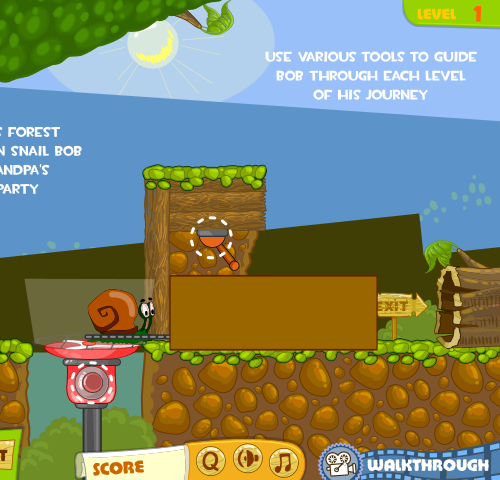
\includegraphics[height=1.33in]{teaser_flash.png}
  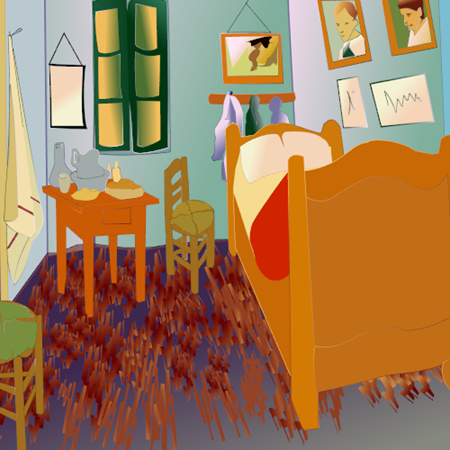
\includegraphics[height=1.33in]{teaser_vangogh.png}
  
\includegraphics[height=1.33in]{teaser_siggraph.png}
  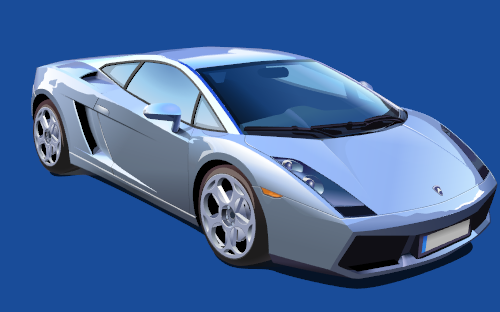
\includegraphics[height=1.33in]{teaser_car.png}
  \caption{\label{fig:teaser} GPU-accelerated scenes rendered at super-real-time rates with
  our system:
 Snail Bob Flash-based game (5ms) by permission of Andrey Kovalishin and Maxim Yurchenko,
 Van Gogh SVG scene with gradients
  (5.26ms) by permission of Enrique Meza C, complete (shown clipped) SIGGRAPH web page (4.8ms), and SVG scene with path
  clipping (1.9ms) by permission of Michael Grosberg, all
  rendered on a GeForce 560M laptop.}

}

%% The ``\maketitle'' command must be the first command after the
%% ``\begin{document}'' command. It prepares and prints the title block.

\maketitle

%\makeatletter
%\preto{\@verbatim}{\topsep=0pt \partopsep=0pt }
%\preto{\@lstlisting}{\topsep=0pt \partopsep=0pt }
%\makeatother

%% Abstract section.

%\vspace{-10pt}


\begin{abstract}

For thirty years, resolution-independent 2D standards (e.g. PostScript,
SVG) have depended on CPU-based algorithms for the filling and
stroking of paths.  Advances in graphics hardware have largely
ignored accelerating resolution-independent 2D graphics
rendered from paths.

We introduce a two-step ``Stencil, then Cover'' (StC) programming
interface.  Our GPU-based approach builds upon existing techniques for curve
rendering using the stencil buffer, but we {\em explicitly} decouple
in our programming interface the {\em stencil step} to determine
a path's filled or stroked coverage from the subsequent {\em cover
step} to rasterize conservative geometry intended to test and reset the
coverage determinations of the first step while shading color samples
within the path.  Our goals are completeness, correctness, quality, and
performance---yet we go further to unify path rendering with OpenGL's
established 3D and shading pipeline.  We have built and productized our
approach to accelerate path rendering as an OpenGL extension.

\end{abstract}



%% ACM Computing Review (CR) categories. 
%% See <http://www.acm.org/class/1998/> for details.
%% The ``\CRcat'' command takes four arguments.
\begin{CRcatlist}
  \CRcat{I.3.2}{Computer Graphics}{Graphics Systems}{Stand-alone systems};
\end{CRcatlist}

%% The ``\keywordlist'' command prints out the keywords.
\keywordlist

\TOGlinkslist


\section{Introduction}
\label{sec:intro}

%% The ``\copyrightspace'' command must be the first command after the 
%% start of the first section of the body of your paper. It ensures the
%% copyright space is left at the bottom of the first column on the first
%% page of your paper.

\copyrightspace

When people surf the web, read PDF documents, interact with smart
phones or tablets, use productivity software, play casual games, or
in everyday life encounter the full variety of visual output created
digitally (advertising, books, logos, signage, etc.), they are experiencing
resolution-independent 2D graphics.

While 3D graphics dominates graphics research, we observe that most visual
interactions between humans and computers involve 2D graphics.  Sometimes
this type of computer graphics is called {\em vector graphics}, but we
prefer the term {\em path rendering} because the latter term emphasizes
the path as the unifying primitive for this approach to rendering.

\subsection{Terminology of Path Rendering}

A {\em path} is a sequence of trajectories and contours.  In this context,
a {\em trajectory} is a connected sequence of {\em path commands}.
Path commands include line segments, B\'{e}zier curve segments, and
partial elliptical arcs.  Each path command has an associated set of
numeric parameters known as {\em path coordinates}.  When a pair of path
coordinates defines a 2D $(x,y)$ location, this pair is a {\em control
point}.  Intuitively a trajectory corresponds to pressing a pen's tip
down on paper, dragging it to draw on the paper, and eventually lifting
the pen.

A {\em contour} is a trajectory with the same start and end point; in other
words, a closed trajectory.  These contours and trajectories may be
convex, self-intersecting, nested in other contours, or may intersect
other trajectories/contours in the path.  There is generally no bound
on the number of path segments or trajectories/contours in a path.
For a rendering ``primitive,'' paths can be quite complex.

Paths are rendered by either {\em filling} or {\em stroking} the path.
Conceptually, path filling corresponds to determining what points
(framebuffer sample locations) are logically ``inside'' the path.
Stroking is roughly the region swept out by a fixed-width pen---centered
on the trajectory---that travels along the trajectory orthogonal to the
trajectory's tangent direction.

\subsection{History, Standards, Motivation, and Contributions}

Seminal work by Warnock and Wyatt
\shortcite{Warnock:1982:DIG:800064.801297} introduced a coherent model
for path rendering.  Since that time, many standards and programming
interfaces have incorporated path rendering constructs into their
2D graphics framework.  Without being exhaustive, we note
%\vspace{-4pt}
\begin{itemize}
\item {\em document presentation and printing}: PostScript \cite{PLRM}, PDF \cite{PDF-Spec}
\item {\em font specification}: PostScript fonts \cite{Type1-Spec}
\item {\em immersive web}: Flash \cite{SWF-File-Format}, HTML 5's Scalable Vector Graphics \cite{SVG-Spec}
\item {\em 2D programming interfaces}: OpenVG \cite{OpenVG-Spec}
\item {\em productivity software}: Illustrator, Photoshop, Office
\end{itemize}
%\vspace{-1pt}
Despite path rendering's 30 year heritage and broad adoption, it has
not benefited from acceleration by graphics hardware to anywhere near 
the extent 3D graphics has.  Most path rendering today is performed
by the CPU with sequential algorithms, not particularly different from
their formulation 30 years ago.  Our motivation is to harness {\em existing}
GPUs to improve the overall experience achievable with path rendering.

We present a productized system for GPU-accelerated path rendering in
the context of the OpenGL graphics system; see some of our rendering results
in Figure~\ref{fig:teaser}.  Our system works on the three most-recent
architectural generations of GeForce and Quadro GPUs---and we expect
all recent GPUs can support the algorithms and programming interface
we describe.

The primary contributions delivered by our system are:
%\vspace{-4pt}
\begin{itemize}
  \item A novel "stencil, then cover" programming interface
  for path rendering, well-suited to acceleration by GPUs.
  \item Our programming interface's efficient implementation within the
  OpenGL graphics system to avoid CPU bottlenecks.
  \item Accompanying algorithms to handle tessellation-free stenciled stroking 
  of paths, standard stroking embellishments such
  as dashing, clipping paths to arbitrary paths, and mixing 3D and path
  rendering.
\end{itemize}
%\vspace{-1pt}
Section~\ref{sec:prior} reviews prior path rendering systems.
Section~\ref{sec:approach} explains our approach;
we cite the crucial prior research that our approach integrates in this section.
Section~\ref{sec:discuss} compares our quality and performance to other
implementations and highlights our system's novel ability to mix with 3D
and GPU-shaded rendering.  Section~\ref{sec:future} discusses opportunities for
future work.

\subsection{New Demands on Path Rendering}

Historically, applications mostly ``pre-render'' 2D content specified
with paths into bitmaps for glyphs and icons/images for vector artwork,
then cache and blit those rasterized results as needed.  Rendering
directly from the path data generally proved too slow to be viable.
Early window systems based on path rendering concepts such as Sun's NeWS
\cite{NeWS-Book} and Adobe's Display PostScript \cite{DisplayPostScript}
were arguably overly ambitious in basing their 2D rendering model around
path rendering rather than resolution-dependent 2D bitmap rendering as
did the more successful GDI and X11-based systems that proved easier
for 2D graphics hardware to accelerate.

\subsubsection{Increasing Screen Density and Resolution}

Smart phones and tablets have created new platforms
free from legacy display limitations such as relatively low---by today's available technology---display density
(measured in {\em dots-per-inch} or DPI) and the dated visual appearance established
by resolution-dependent bitmap graphics.  
Apple's new iPad display has a display density of 264 DPI, greatly surpassing
the 100 DPI density norm for PC screens.  These handheld devices
are carried directly on one's person so their screen real estate is
relatively fixed---so improvements in display appearance is likely to
be through increasing screen density rather than enlarging screen area.

Pixel resolutions for conventional monitors are increasing too.
Large 2560x1600 resolution screens are mass-produced and readily
available.  Driving such high resolutions with CPU-based path rendering
schemes is untenable at real-time rates.  Indeed the very heterogeneity of modern displays in terms of
pixel resolution, screen size, and their combination---pixel
density---strengthens the case for improving path rendering performance.

\subsubsection{Multi-touch Interfaces}

Mobile devices also rely on multi-touch screens for input so the user is
extremely aware of the latency between touch gestures and the resulting
screen update.  The user is literally pointing at the pixels they expect
to see updated.  Multi-touch encourages rotation and scaling.
When imagery can easily be rotated, scaled, sub-pixel translated, and even
projected, assumptions that all text and graphics will be orthographically aligned to
the screen's pixel grid are no longer a given so
rendering all path content directly from paths makes sense.

\subsubsection{Immersive Web Standards}

The proximate HTML 5 web standard exposes path rendering functionality
in a standard and pervasive way through both Scalable Vector Graphics (SVG)
and the Canvas element.

JavaScript performance has increased to the point that dynamic content
can be orchestrated within a standards-based HTML 5 web page such that
the system's path rendering performance is often a bottleneck.

\subsubsection{Power Wall}

Minimizing power consumption has become a mantra for computer system
design across all classes of devices---whether mobile devices or not.
When power is at a premium, moving CPU- and bandwidth-intensive
computations such as pixel manipulation and rasterization to
more power-efficient GPU circuitry can reduce overall power
consumption while improving interactivity and minimizing update latency.
GPU-acceleration of path rendering is precisely such an opportunity.



\begin{figure*}[t!]
        \center{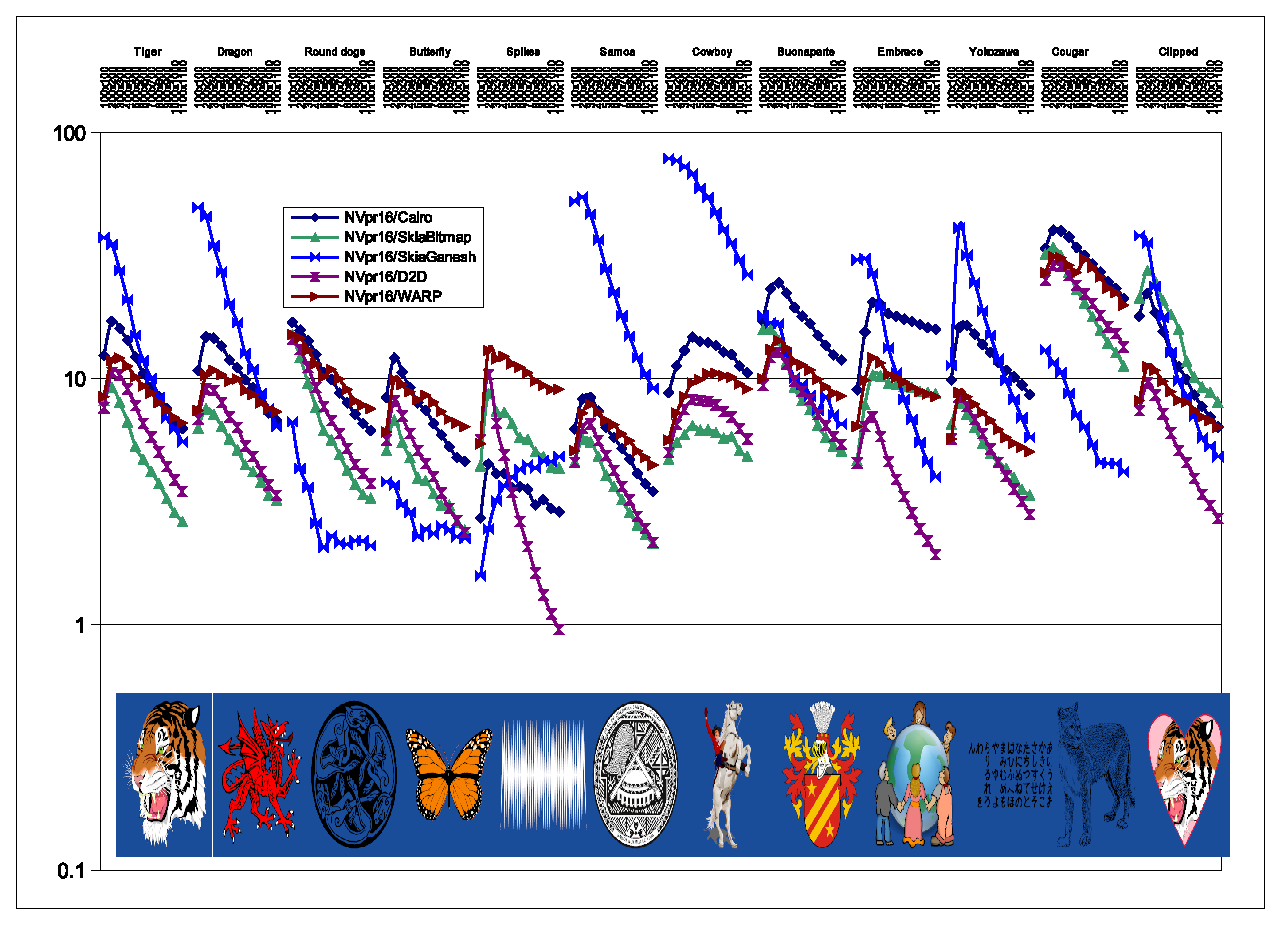
\includegraphics[width=6.99in,height=3.2in]{nvpr_performance.eps}}
        \caption{\label{fig:nvpr-performance} Performance ratios rendering SVG content at window resolutions from $100^2$ to $1100^2$.
  A ratio of 1.0 means the {\tt NV\_path\_rendering} (16 samples per pixel) performance is equal to the other renderer; higher ratios indicate how many multiples faster {\tt NV\_path\_rendering} is than the alternative.  Note the logarithmic Y axis.  Scenes were selected for their variety.  Benchmark configuration is a GeForce 650 and fast Core i7 CPU.}
\end{figure*}


\section{Prior Path Rendering Systems}
\label{sec:prior}

\subsection{CPU-based Path Rendering Systems Critiqued}

Path rendering is historically and still typically performed by
CPU-based scan line renderers.  Paths are converted into a set of edges.
These edges are transformed and sorted in Y-order.  Then the edges are
intersected with each scan line, sorted in X-order, and pixels in the
path region are updated.

The scan-line rendering approach is notable for being work-efficient
and cache-friendly.  No computation is expended on pixels that are
obviously outside the path and only active edges are considered when
processing a given scan line.  Such scan line renderers use a ``chunker''
strategy---where rather than the chunk being a 2D tile, the chunk is a
single scan line.  This leads to a reasonably friendly access pattern for
CPU caches.  Additionally the scan line enter/leave counts are transient.
In contrast to a window-sized ancillary buffer such as a depth or stencil
buffer, the scan line enter/leave counts can live in the cache and have
their storage recycled for each processed scan line.

While work-efficient {\em and} cache-friendly as noted, this CPU-intensive
approach is quite sequential.  Every path must be transformed into screen
space.  Every path must be scan line rasterized.  Every scan line must
be intersected with the active edge list.  Every sorted active edge list
must be scanned left-to-right.  There is not an easy way to pipeline
all these tasks or exploit massive parallelism---such as is routine for
GPU-accelerated 3D graphics.  Hence this is an approach that maps well
to the CPU but cannot be obviously accelerated in this form by the GPU.

\subsection{GPU-based Path Rendering Systems}

Over the years, many attempts have been made---with varying degrees of
mixed success---to accelerate path rendering with GPUs.
We postpone discussion of prior techniques for GPU rendering of curves with the stencil buffer
to Section~\ref{sec:approach} since they are the basis for our approach.

\subsubsection{Acceleration of Path Rendering Programming Interfaces}

Cairo \cite{Rejected} is an open-source path rendering implementation.
An early attempt at GPU-acceleration called Glitz \cite{Glitz} has
since been abandoned.  Glitz operated at the level of the XRender
\cite{Packard:2001:DIX:647054.715760} extension so did not accelerate
paths directly.  Arguably, Glitz was a more GPU-assisted back-end than
GPU accelerated. 
More recently, Cairo has worked on a first-class GPU back-end but the
immediate mode nature of the Cairo API and converting CPU-transformed
paths to spans limits the acceleration opportunities.  

Microsoft's Direct2D \cite{Direct2D} API is layered upon Direct3D.
Direct2D operates by transforming paths on the CPU and then performing
a constrained trapezoidal tessellation of each path.  The result is a
set of pixel-space trapezoids and additional shaded geometry to compute
fractional coverage for the left and right edges of the trapezoids.
These trapezoids and shaded geometry are then rasterized by the GPU.
The resulting performance is generally better than entirely CPU-based
approaches and requires no ancillary storage for multisample or stencil
state; Direct2D renders directly into an aliased framebuffer with
properly antialiased results.  Direct2D's primary disadvantage is the
ultimate performance is determined not by the GPU (doing fairly trivial
rasterization) but rather by the CPU performing the transformation and
trapezoidal tessellation of each path and Direct3D validation work.

Skia is the C++ path rendering API used by Google's Android and Chrome
browsers.  Skia has a conventional CPU-based path renderer but has
recently integrated a new OpenGL ES2-accelerated back-end called Ganesh.
Ganesh has experimented with two accelerated approaches.  The first
used the stencil buffer to render paths.  Because of API overheads
with this approach, this first approach was replaced with a second
approach where the CPU-based rasterizer computes a coverage mask which
is loaded as a texture upon every path draw to provide the GPU proper
antialiased coverage.  This hybrid scheme is often bottlenecked by the
dynamic texture updates required for every rendered path.

The Khronos standards body worked to develop an API standard known
as OpenVG with the explicit goal of enabling hardware-acceleration of
path rendering (the {\em VG} stands for vector graphics).
Various companies and research groups have worked to develop OpenVG
hardware designs \cite{iMX35,Huang:2006:IOR:1169227.1169771,4637621} that,
based on available descriptions, are fairly similar to the conventional
CPU-based scan line rasterizer scheme, recast as a hardware unit.
Reported performance levels are quite low compared to what we report.

\subsubsection{Vector Texture Schemes}

An unconventional approach to GPU-accelerating path rendering
is cleverly encoding path content into GPU memory---typically as a
texture---and then using a programmable shader essentially to decode the
path content.  Nehad and Hoppe \shortcite{Nehab:2008:RRG:1457515.1409088}
and Qin \shortcite{QinThesis} adopt variations on this approach.  While this
approach has some interesting advantages such as being able to directly
``texture map'' 3D geometry with path rendered content, these approaches
suffer from the need to preprocess a static path scene into a specific
texture encoding.  This makes this approach unsuitable for editable or
dynamic path rendering.  Additionally, many rendering approximations
and authoring limitations are needed to make vector texture schemes
tractable.

\subsubsection{Discussion of Deficiencies}

The norm for CPU-based path rendering systems is maintaining roughly
16 coverage samples per pixel (details vary).  This creates a challenge
for GPU-based schemes because GPUs often support 1, 2, 4, or 8 samples
per pixel through multisampling.  This often creates a situation where
the GPU-accelerated path rendering is inferior to the CPU-based path
rendering quality.

When path rendering schemes are layered upon existing OpenGL or Direct3D
APIs, we have observed performance being limited by the state change
rate of the underlying 3D API.  Often path rendering can result in
many state changes per path when scenes can easily consist of 100s or
1000s of paths.  In this case, the API overhead can substantially limit
the overall performance.  Our experience studying prior approaches to
using GPUs for path rendering indicates these approaches are often more
GPU-assisted rather than GPU-accelerated, with this attributable to
continuous CPU involvement or substantial CPU-based preprocessing.




\section{Our Approach}
\label{sec:approach}

In contrast to other systems for accelerating path rendering with GPUs,
our approach {\em explicitly} reveals the coverage determinations.  These
determinations---for both filling and stroking---appear as stencil buffer
updates.
A crucial insight underlying our approach is never determining the
boundary between the ``inside'' and ``outside'' of a stroke or fill.
Instead, we rely on point-sampled determinations of whether a particular
$(x,y)$ framebuffer location is inside or outside the stroke or fill.  For antialiasing, we rely on GPU
multisampling to provide multiple sample coverage positions, each with
its own sub-pixel stencil value.

\subsection{Stencil, then Cover}

We perform path rendering in two steps.  This is not unique; {\em all} path
rendering schemes involve two steps.  The two steps may be ``tessellate,
then render tessellation'' \cite{Direct2D} or ``intersect with scan
line, then paint pixels'' \cite{Rejected} or ``ray cast, then shade''
\cite{Nehab:2008:RRG:1457515.1409088} but each rendering of a path is
inherently sequential in the sense that determining what pixels are
covered must precede shading and blending those pixels.

What is novel in our approach is {\em explicitly} decoupling the two
steps.  We call our approach, with its two decoupled steps, ``Stencil, then Cover'' (StC).
Rather than a single {\tt DrawPath} operation that hides the two-step nature
of path rendering within the implementation, an OpenGL application
using our extension first ``stencils'' the path in the stencil buffer
\cite{Kurt:1995:ieeestyle}, then ``covers'' the path to shade it.

This explicitly decoupled approach has advantages not available
in interfaces that appear to offer a one-step {\tt DrawPath} command.
Our two-step approach makes arbitrary path clipping, mixing with 3D
graphics, programmable blend modes, and other novel path rendering usages
possible.

\subsection{Filling}

\subsubsection{Improvements to Prior Methods}

Our approach to filling paths is inspired by the work of Loop and Blinn
\shortcite{Loop:2005:RIC:1186822.1073303} who developed an efficient fragment
shader-based approach to determining whether or not an $(x,y)$ sample is
inside or outside a given quadratic or cubic B\'{e}zier hull.  In the
Loop-Blinn formulation, inexpensive arithmetic on interpolated texture
coordinates provides a Boolean predicate which when true indicates the
fragment's sample position is not inside the B\'{e}zier region.

Our approach is {\em not} the first time the stencil buffer has been utilized
for stenciling paths.  Kokojima et al. \shortcite{Kokojima:2006:RIR:1179849.1179997} applied
the Loop-Blinn scheme in conjunction with the stencil buffer to
determine the winding number of TrueType glyph outlines.  Kokojima
et al. showed the general filled polygon algorithm of Lane et
al. \shortcite{Lane:1983:AFR:357323.357326}---subsequently popularized for
use with the stencil buffer \cite{RedBook}---can naturally combine with
the Loop-Blinn quadratic discard shader to determine the samples inside
an arbitrarily complex TrueType outline.  After stenciling each glyph
into the stencil buffer, conservative geometry based on a convex hull or
bounding box can test against the non-zero stencil values, shade those
samples, and reset the stencil values back to an initial zero state.

Kokojima's approach does not immediately extend to cubic B\'{e}zier
segments because the inside region within a cubic B\'{e}zier hull is not
necessarily convex.  Rueda et al. \shortcite{Rueda:2008:TSG:1411846.1411922}
addressed this by providing simple topological strategies to subdivide
cubic B\'{e}zier hulls using B\'{e}zier subdivision to guarantee
convexity, but used an overly expensive discard fragment shader based
on B\'{e}zier normalization rather than applying the Loop-Blinn cubic
formulation.

Our approach to handling cubic B\'{e}zier segments builds on all this
work by combining cubic B\'{e}zier convex subdivision rules with the
Loop-Blinn cubic formulation.  We also perform the discard shaders at
sample-rate rather than pixel-rate for improved coverage determinations
and antialiasing. We use interpolation at explicit sample positions and
our target GPU's sample mask functionality to evaluate multiple samples
within a pixel in a single shader instance.

PostScript, SVG, and other standards support partial circular and
elliptical arcs so an additional discard shader, expressed in Cg, handles
these cases:
\label{round-coverage-shader}
%\vspace{-3pt}
\begin{lstlisting}
void roundCoverage(float2 st : TEXCOORD0.CENTROID)
{
  if (st.s*st.s + st.t*st.t > 1) discard;
}
\end{lstlisting}
%\vspace{-1em}
with the $(s,t)$ texture coordinates assigned so (0,0) is centered
at the origin of roundness to discard
samples outside the arc region contained in a sequence of one or more
polygonal hulls bounding such arcs.

\subsubsection{Baked Form of Filled Paths}

In order to render a filled path, we ``bake'' the path into a
resolution-independent representation from which the path can be stenciled
under arbitrary projective transforms.  This baking process takes time
linearly proportional to the number of path commands.  The resulting baked
path data resides completely on the GPU.  The required GPU storage is
also linearly proportional to the number of path commands.  For a static
path, the baking process needs to be done just once; the baking process must
be repeated if the path's commands or coordinates change, but edits to
the path, including insertions and deletions of commands, require just
re-baking the path segments at or immediately adjacent to the edits.

Once baked, a filled path is reduced to five sets of primitives:
%\vspace{-3pt}
\begin{enumerate}
  \item Polygonal anchor geometry (structured as triangle fans), rendered
  with no shader.
  \item Quadratic discard triangles, rendered with a Loop-Blinn quadratic
  discard shader.
  \item Cubic discard triangles (if the cubic B\'{e}zier hull is a
  triangle) and quadrilaterals, rendered with a Loop-Blinn cubic discard
  shader.
  \item Arc discard triangles, rendered with the {\tt roundCoverage}
  discard shader shown above.
  \item Conservative covering geometry, typically a triangle fan or
  quadrilateral.
\end{enumerate}
Primitive sets \#1 through \#4 are rendered during the stencil fill step.  Two-sided stencil testing increments non-discarded stencil samples of front-facing primitives; back-facing primitives instead decrement non-discarded stencil samples.
Primitive set \#5 is rendered during the cover fill step.  Primitive sets
\#2 through \#4 have properly assigned texture coordinates that drive
each set's respective discard shader.  Figure \ref{fig:filling-explained}
visualizes the baked anchor, discard, and cover geometry.

\begin{figure}[tb]
  %\center{
\includegraphics[width=\columnwidth]{filling_explained.eps}}
  \center{
\includegraphics[width=3.3in]{filling_explained.eps}}
  \caption{\label{fig:filling-explained} Filled path, with control
  points, with anchor geometry, and with cubic B\'{e}zier discard hulls,
  and conservative cover geometry.}
\end{figure}
 
This approach to path filling is theoretically sound because the stencil
rendering reduces to a winding number computation consistent with a discrete
formulation of Jordan's Theorem \cite{625138}.

All the data for a baked path can be stored within a single allocation of
GPU memory to minimize the expense of stenciling or covering the path.
Because the baked representation is completely resolution-independent,
robust, and entirely on the GPU, the CPU overhead to launch the stenciling
and/or covering of an already baked path object is minimal.

%By implementing our approach as an OpenGL extension---named {\tt
%NV\_path\_rendering} \cite{NVpr}, performing the stencil and cover steps
%avoids the API and driver validation overhead (explained in
%Section~\ref{sec-performance}) that has plagued other GPU-based approaches
%to path rendering.

We implement our approach as an OpenGL extension named {\tt
NV\_path\_rendering} \cite{NVpr}.  Performing the stencil and cover steps
within the graphics driver avoids
the API and driver validation overhead (see
Section~\ref{sec-performance}) that plagued other GPU-based approaches.
Figure~\ref{fig:pipelines}
shows how our new path pipeline co-exists with the existing pipelines
in OpenGL for pixel and vertex processing.

\begin{figure}[tb]
  %\center{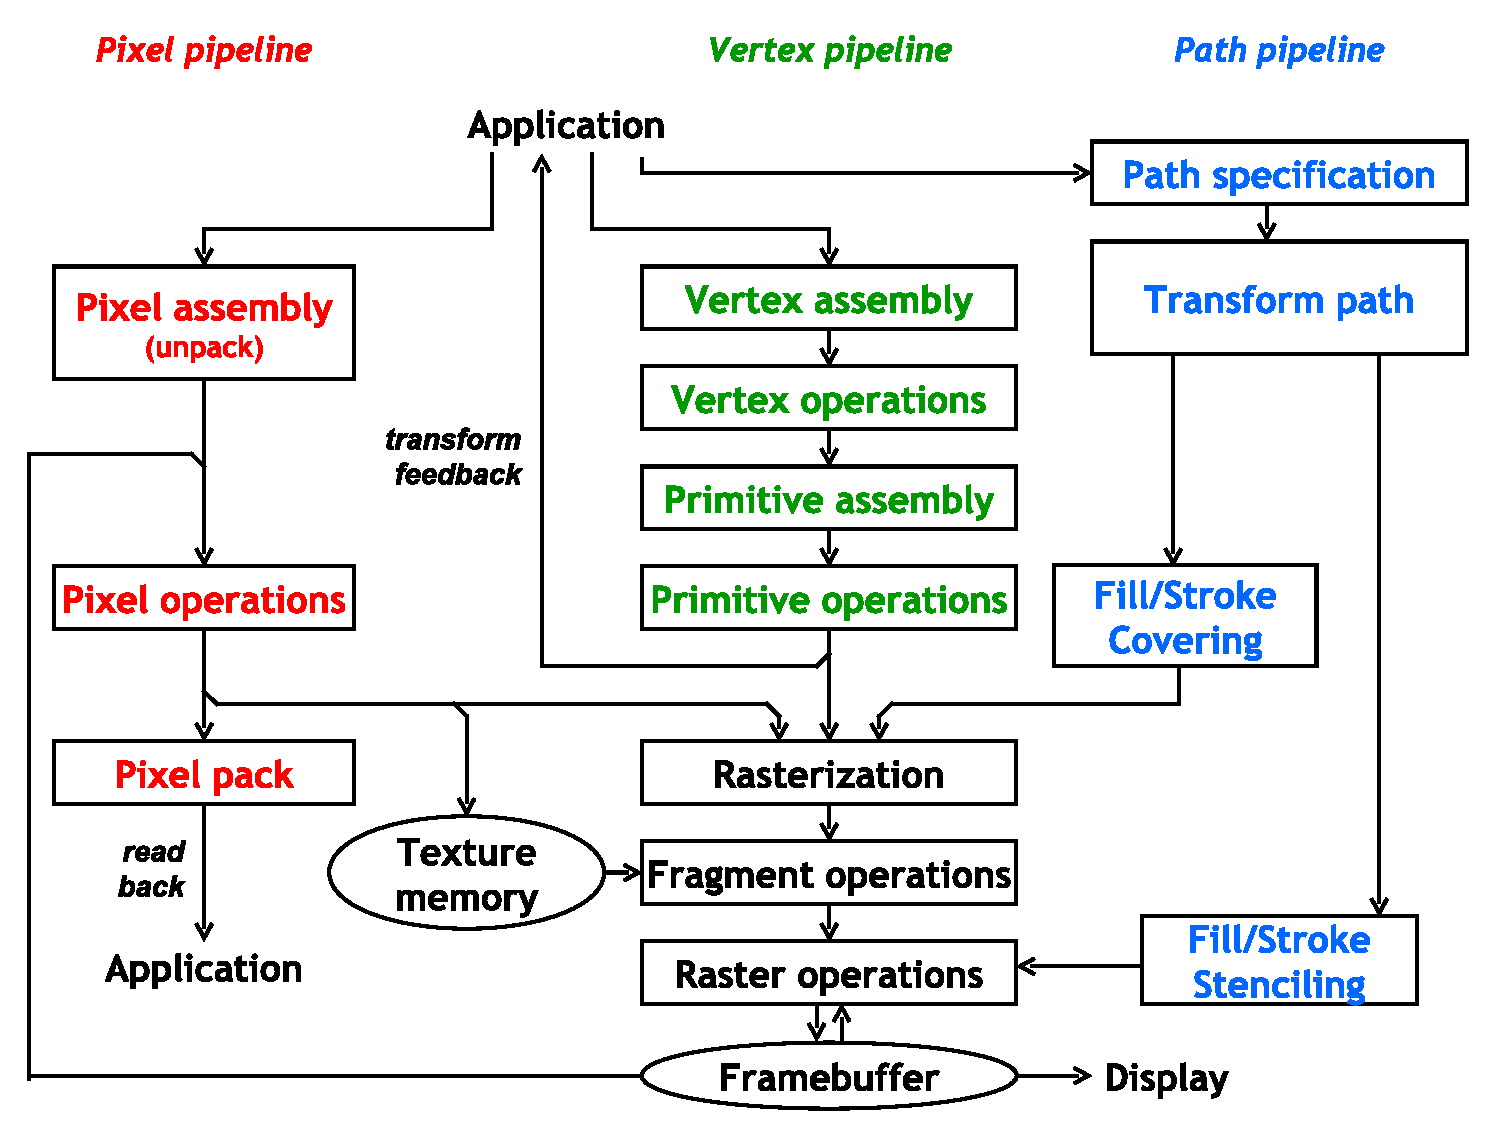
\includegraphics[width=\columnwidth]{pipelines.eps}}
  \center{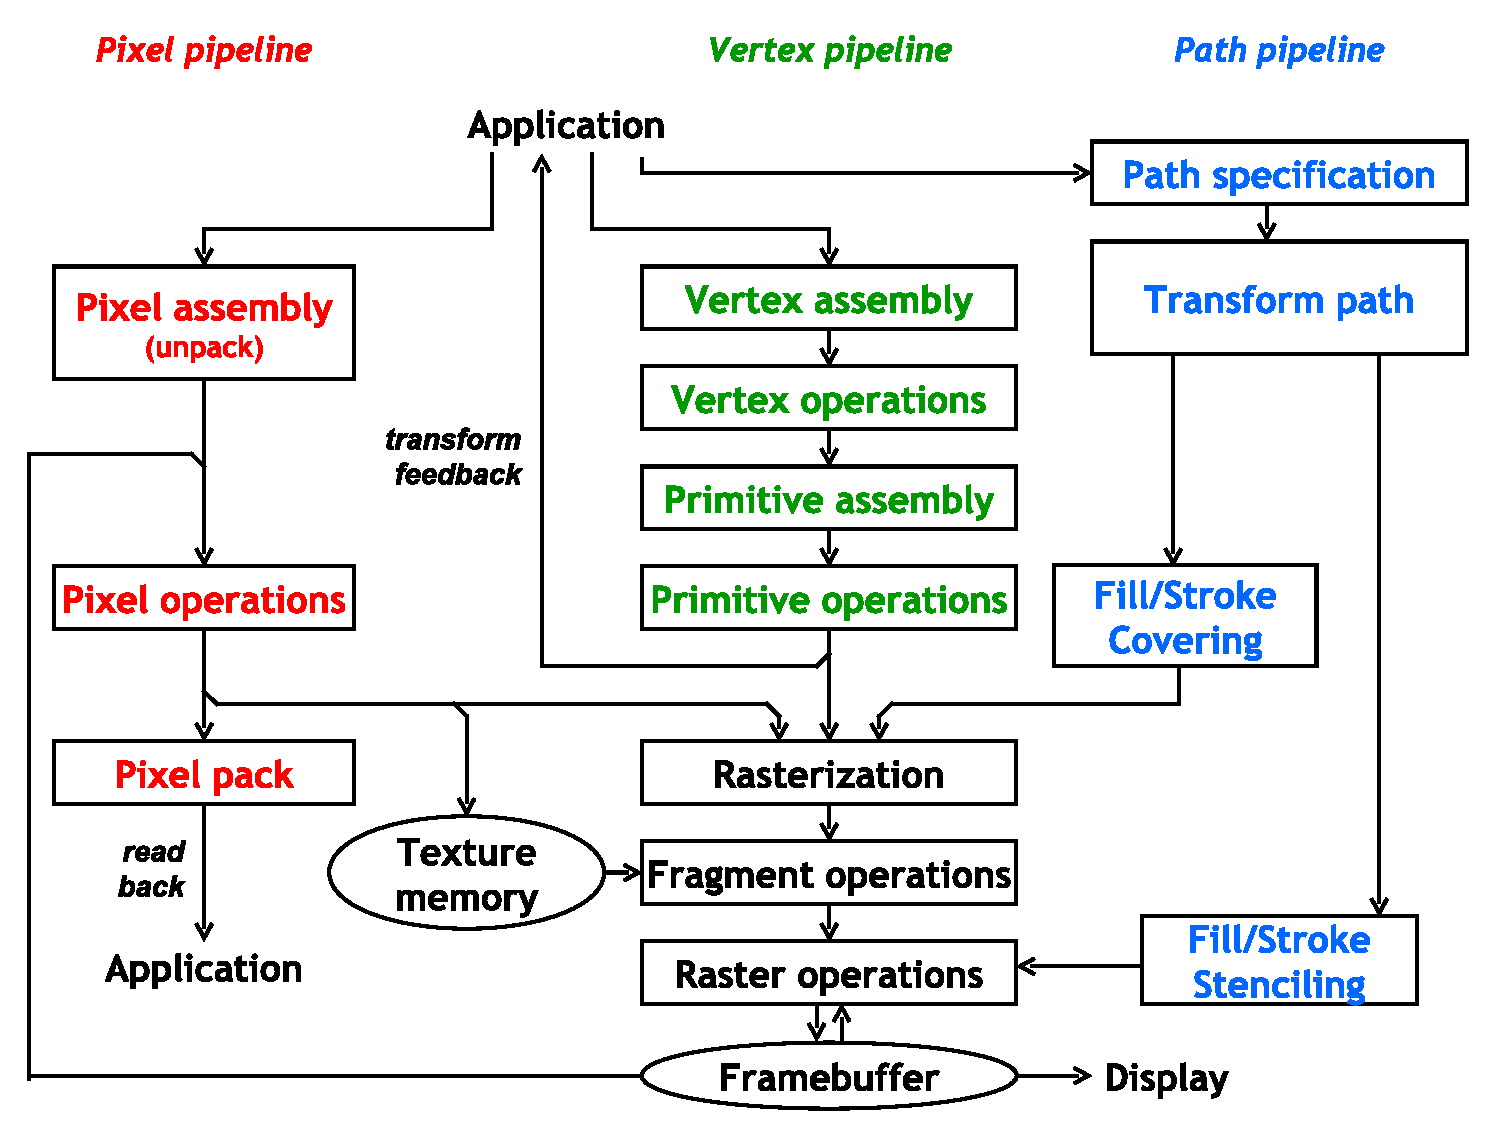
\includegraphics[width=2.8in]{pipelines.eps}}
  \caption{\label{fig:pipelines} High-level data flow of OpenGL showing
  pixel, vertex, and new path pipelines.}
\end{figure}
 
\subsection{Stroking}

Our stroking approach operates similarly to our filling approach whereby
we stencil, then cover stroked paths from a baked resolution-independent
representation residing on the GPU that requires minimal CPU overhead
to both stencil and cover.

\subsubsection{Quadratic B\'{e}zier Stroking}

Analytically determining the points contained by a stroke curved
segment is \underline{not} easy.  The boundary of the stroked region
of a quadratic B\'{e}zier corresponds to an offset curve.  While the
quadratic B\'{e}zier curve generating the offset curve is \nth{2} order,
the offset curve for this generating segment's boundary is \nth{6} order
\cite{Salmon}.  This makes exactly determining an intersection with
this boundary unfeasible, particularly within the execution context
of a GPU's fragment shader.  The boundary becomes even more vexing for
partial elliptical arcs and cubic B\'{e}zier segments.  The boundary for
a general cubic B\'{e}zier curve is \nth{10} order \cite{Farouki1990101}!

\paragraph{Quadratic B\'{e}zier Segment Point Containment}

Hence our approach involves simply determining if a given $(x,y)$ point is
inside or outside the stroked region of a quadratic B\'{e}zier segment.
This can be reduced to solving a \nth{3} order equation.

A quadratic B\'{e}zier segment $Q$---defined by the segment's three
control points $C_0$, $C_1$, and $C_2$---can converted to monomial
form $Q(t)=At^{2}+Bt+C=0$ for $t \in [0,1]$.  A point $P$ is judged
within the stroke of $Q$ when there is a parametric value $s$ on $Q$
such that $Q'(s) \cdot (P-Q(s))=0$ and the squared distance between $Q(s)$ and
$P$ is within the squared stroke radius.  (The dot product of a quadratic
function and the derivative of a quadratic function is \nth{3} order.)
Intuitively this corresponds to finding the 1 or 3 points $Q(s)$ with
a tangent direction orthogonal to the segment connecting $P$ and $Q(s)$.
Such solutions $s$ will be local minima or maxima for the distance between
$P$ and points on $Q$ so computing the squared distance $d=(Q(s)-P) \cdot
(Q(s)-P)$ for each solution $s$ indicates if $P$ is within the stroke of
$Q(t)$ for $t \in [0,1]$ when both $s \in [0,1]$ and $d$ is less than or
equal the square of half the path's stroke width.  Figure~\ref{fig:quadratic-stroke} visualizes this procedure.

\begin{figure}[t]
  %\center{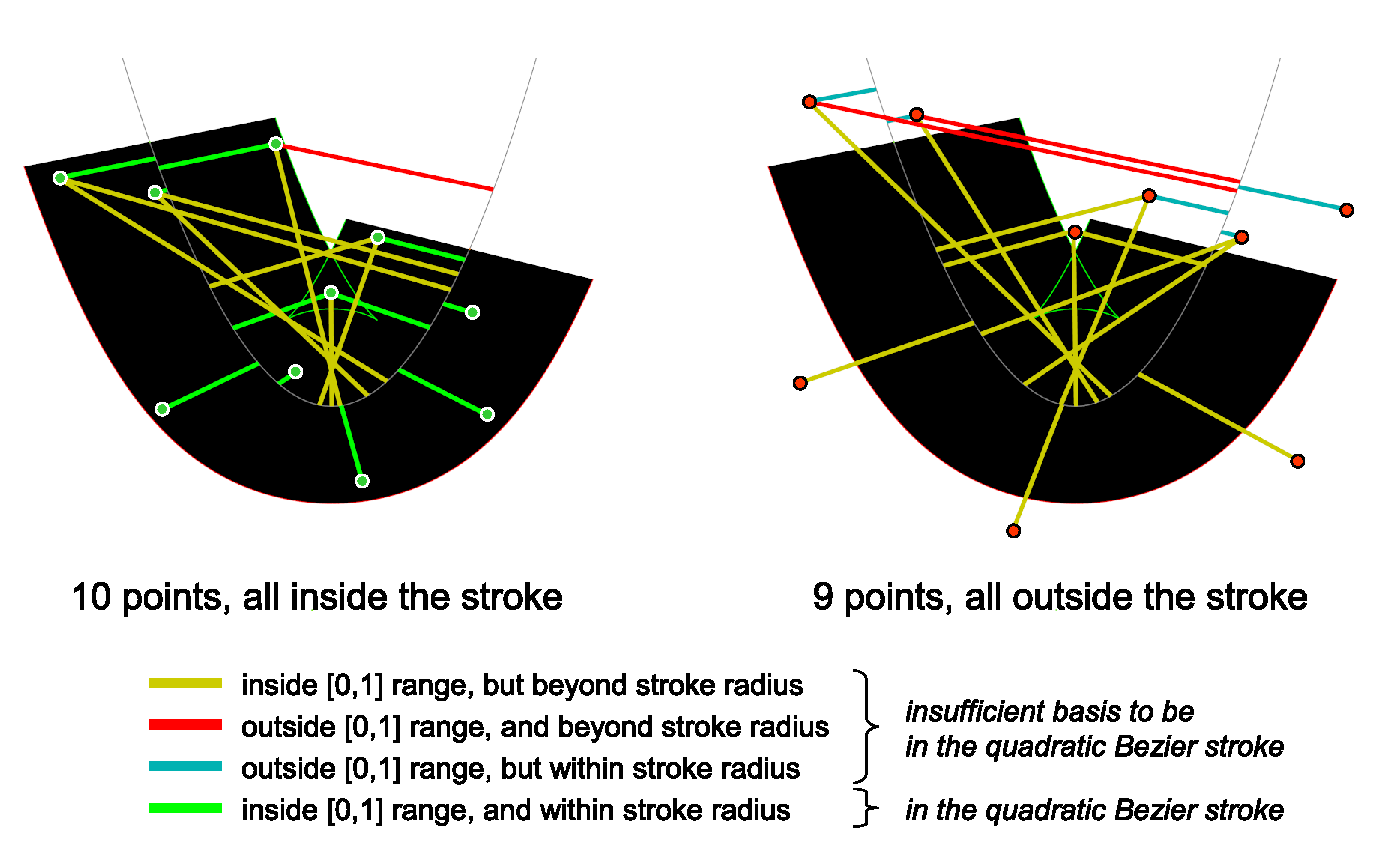
\includegraphics[width=\columnwidth]{quadratic_stroke.eps}}
  \center{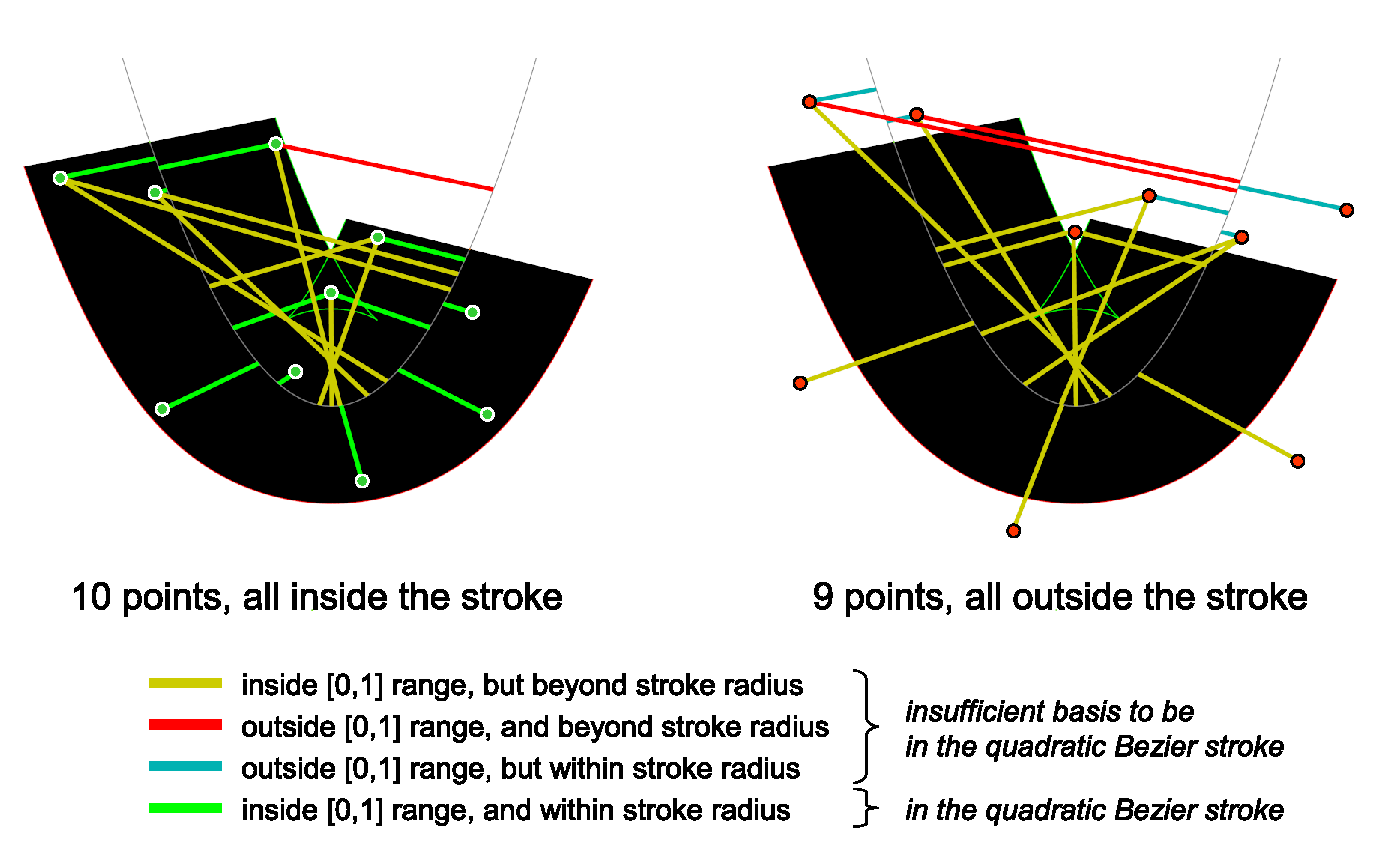
\includegraphics[width=3.3in]{quadratic_stroke.eps}}
  \caption{\label{fig:quadratic-stroke} Visualization of points within
  and outside the stroked region of a quadratic B\'{e}zier segment and
  their basis for inclusion or not.}
\end{figure}

Solving the cubic equation at every rasterized sample is expensive,
but the computation can be simplified somewhat.  The cubic equation can
be rearranged into an easier-to-solve depressed cubic \cite{Cardano} of
the form $t^3+G(x,y)t+H(x,y)=0$.  While the coefficients $G(x,y)$ and $H(x,y)$
are different for every path-space $(x,y)$ location, the functions $G$ and
$H$ are linear in terms of $(x,y)$ so a vertex shader can evaluate $G(x,y)$
and $H(x,y)$ at hull positions and exploit the GPU's ability to interpolate
linearly $G$ and $H$ at positions within the hull.

Care is taken when an arrangement of quadratic B\'{e}zier control points
is collinear, collocated, or very nearly so.  In such cases, we demote
the quadratic B\'{e}zier segment to its linear degenerate equivalent
for robustness.

\begin{figure}[t]
  %\center{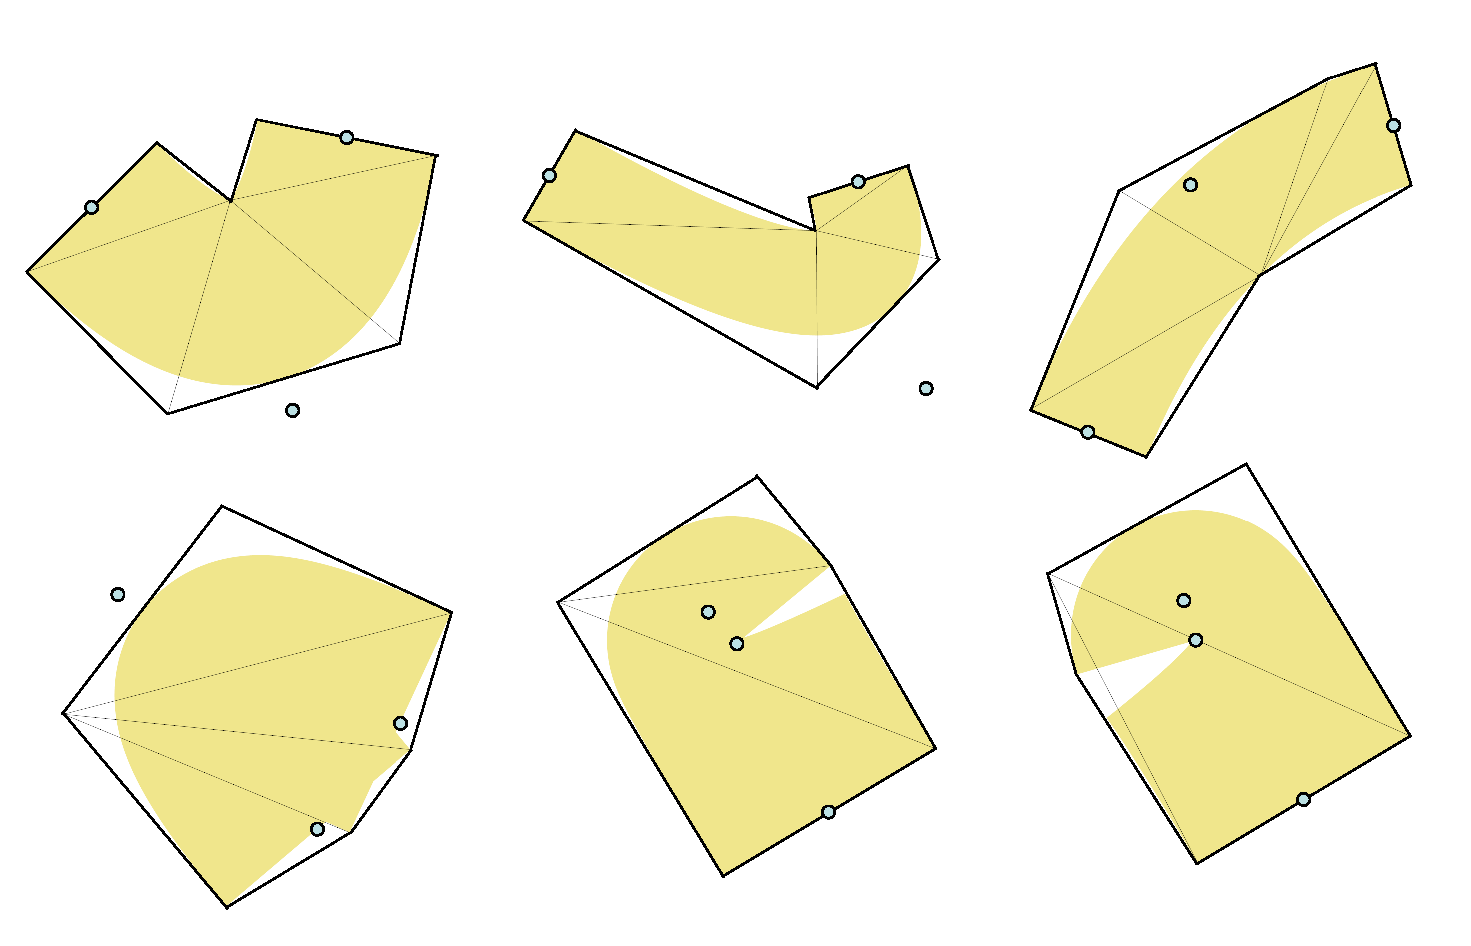
\includegraphics[width=\columnwidth]{quadratic_hull.eps}}
  \center{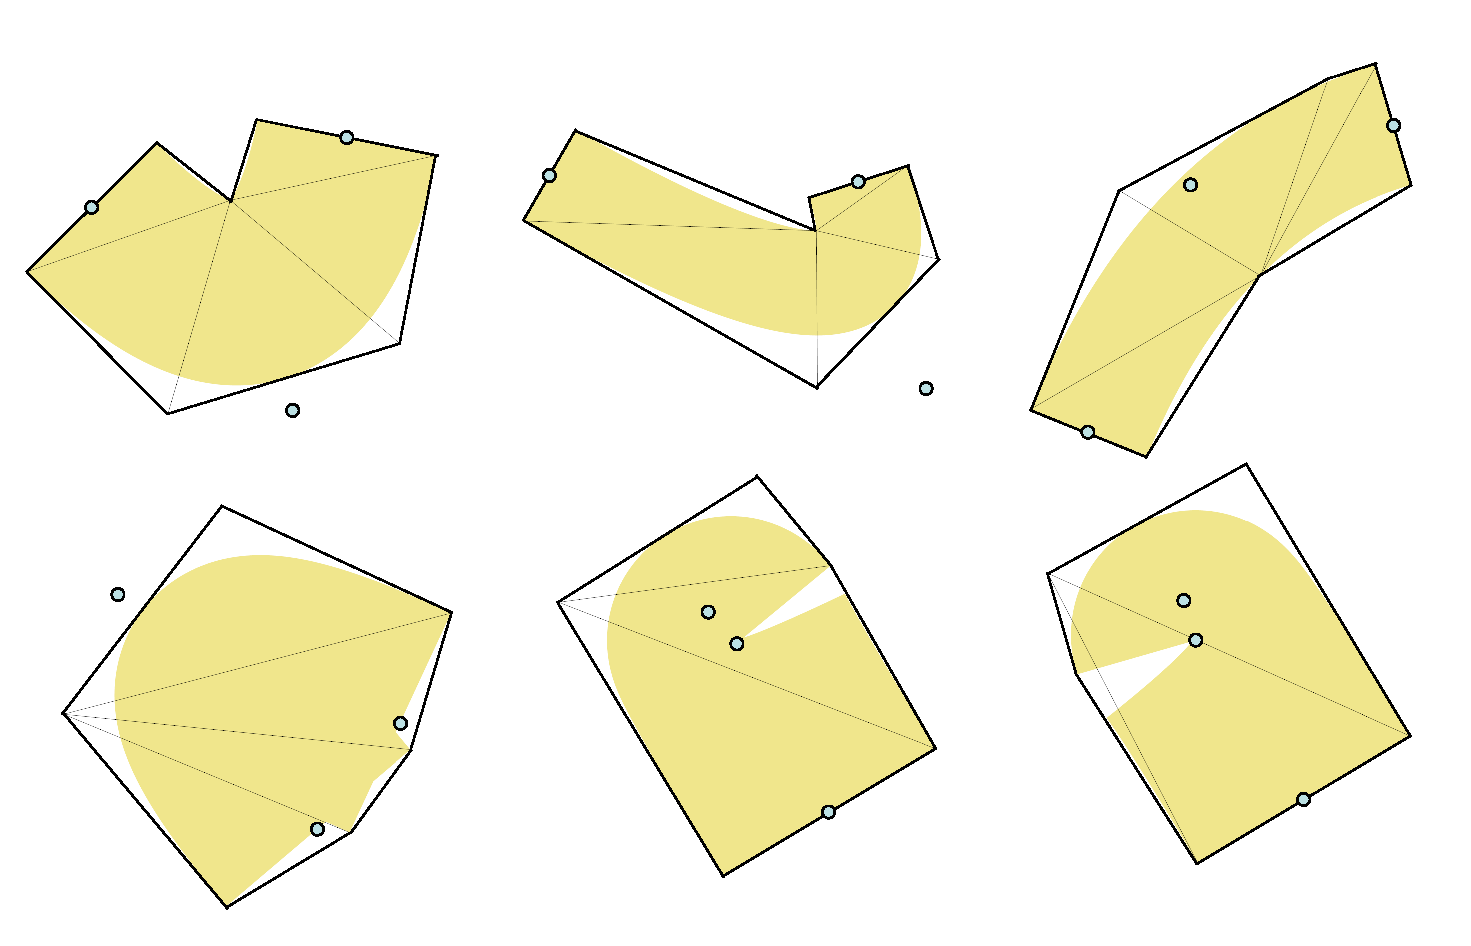
\includegraphics[width=3.3in]{quadratic_hull.eps}}
  \caption{\label{fig:quadratic-hull} Examples of concave (top row)
  and convex (bottom row) stroked quadratic B\'{e}zier segment hulls.}
\end{figure}
 
\paragraph{Stroked Quadratic Segment Hull Construction}

To harness this approach for rendering, we construct a hull
around the quadratic B\'{e}zier stroked segment.  As shown in
Figure \ref{fig:quadratic-hull}, the hull is typically concave,
consisting of seven vertices---though the hull may be convex when
the quadratic stroke's width is wide relative to its arc length.
Ruf \shortcite{Ruf:2011:IBR:2018323.2018346} has addressed the problem of a
tight bounding representation for quadratic strokes, but his approach
involves parabolic edges with the assumption the CPU can evaluate such
edges efficiently; for our purposes, we want a triangular decomposition
of the hull suitable for GPU rasterization.

While solving the cubic equation---even in depressed form---is expensive,
we note that stroked regions are typically small and narrow in screen
space so this expensive process is used sparingly in practice.  Even when
strokes are wide, the massively parallel nature of the GPU makes this
approach quite fast.  Most important to us, once a quadratic stroke
is ``baked'' for rendering, it can be rendered under an arbitrary
linear transformation---including projection---without any further
CPU re-processing.  The hull vertices and their coefficients for $G$
and $H$ can be stored in GPU memory so that stencil-only rendering the
quadratic stroke involves simply configuring the appropriate buffers,
the appropriate vertex and fragment shader pair, and rendering the
hull geometry of the quadratic stroke.

\paragraph{Higher-order-than-Quadratic Stroking}

Path rendering standards incorporate cubic B\'{e}zier segments and
partial elliptical arcs; these involve cubic and rational quadratic
generating curves for rasterized offset curve regions.  The direct
evaluation approach applied to generating quadratic B\'{e}zier curves
is not tractable.

Instead we subdivide cubic B\'{e}zier segments and partial elliptical
arcs into an approximating sequence of quadratic B\'{e}zier segments.
To maintain a curved boundary appearance at all magnifications, our
subdivision approach maintains $G^1$ continuity at quadratic B\'{e}zier
segment boundaries.  No matter how much you zoom into the boundary of
higher-order stroked segments, there is never any sign of linear edges
or even a false discontinuity in the curvature.

Following the approach of Kim and Ahn \shortcite{KimAhn}, we bound the
subdivision such that the true higher-order generating curve never escapes
a specified percentage threshold of the stroke width of the approximating
quadratic stroke sequence.  We also subdivide at key topological features,
specifically points of self-intersection and minimum curvature.

\subsubsection{Stroking Embellishments}

Stroking of line segments, end caps, and joins is straightforward.
Stroked line segments are drawn as stencil-only rectangles.  Polygon
caps (square and triangular) and joins (bevel and miter) are likewise
drawn as stencil-only triangles.  This geometry can be drawn without
any fragment shader.  Round caps and joins are drawn with the same
{\tt roundCoverage} stencil-only sample-rate discard shader (Section
\ref{round-coverage-shader}) used for partial circular and elliptical
arcs for filling with the $(s,t)$ texture coordinates assigned appropriately
to discard samples outside the circular region of the round cap or join.
The baking process for stroked paths includes generating the rectangles
and triangles for line segment and polygonal caps and joins.  Geometry for
round caps and joins is generated along with the texture coordinates to
drive the round coverage discard shader.

\subsubsection{Dashing}

Dashing is a feature of all major path rendering standards except Flash.
Dashing complicates stroking by turning on and off the stroking along
a path based on an application-specified repeating on-off pattern
specified in units of arc length.  Our stroke baking process applies
the dash pattern while gathering the geometry for the stroked path.
While complicated in its details, our dashing process is similar to other
path rendering implementations in its high-level structure.  The primary
difference is curved path segments are reduced to quadratic B\'{e}zier
segments in our approach instead of line segments.  Whereas the arc
length computations in conventional path rendering systems typically
involve recursive subdivision until the curved segment approximates
a line segment, our approach can stop subdividing at
quadratic B\'{e}zier segments.  Unlike higher order curves, the
arc length of a quadratic B\'{e}zier segment (a segment of a parabola)
has a closed form analytical solution:
\begin{eqnarray*}
\lefteqn{ \int _{0}^{1}\!\sqrt {Q_{x}(t)^{2}+ Q_{y}(t)^{2}}{dt} = } \\
&
\frac{\ln ({\frac {b+2\,\sqrt {ac}}{b+2\,c+2\,\sqrt {c\left (c+a+
b\right )}}})\left ({b}^{2}-4\,ac\right )+2\,\left (b+2\,c\right )
\sqrt {c\left (c+a+b\right )}-2\,b\sqrt {ac}}{8c^{3/2}}
\end{eqnarray*}
with copious common subexpressions and 
where $a=B \cdot B$, $b=2B \cdot C$, and $c=C \cdot C$.  Our interest in
this approach is our desire to minimize use of expensive recursive
subdivision algorithms while baking stroked paths, particularly during
dashing.  Some numerical care must be taken to avoid negative square
roots, negative logarithms, and division by zero, but these cases occur
when quadratic segments are nearly linear.
%Using double precision and using Euclidean distance computations when
%control points are collinear---or nearly so---works.

Our dashing approach results in a resolution-independent baked form of
the dashed stroked path.  Once dashed and baked, no further CPU-based
processing is necessary to render dashed paths.  This is in contrast to
other implementations of dashed stroking where dashing has a considerable
CPU processing expense during rendering.  While our implementation must
of course represent each segment resulting from dashing, our render-time
algorithm is completely oblivious to whether the original path was
dashed. 

\subsubsection{Baked Form of Stroked Paths}

Once baked, a stroked path is reduced to four sets of primitives:
%\vspace{-3pt}
\begin{enumerate}
  \item Polygonal geometry (line segments, bevel and miter joins, square
  and triangular end caps) with no shader.
  \item Triangle fans corresponding to quadratic B\'{e}zier segment hulls
  (curved path segments), rendered with a stroked quadratic discard
  shader.
  \item Triangle fans corresponding to round hulls (round end caps and
  joins) rendered with a round coverage shader.
  \item Conservative covering geometry, typically a triangle fan or
  quadrilateral.
\end{enumerate}
Primitive sets \#1 through \#3 are rendered during the stencil stroke
step.  Primitive set \#4 is rendered during the cover stroke step.

The {\tt REPLACE} stencil operation used for stroking is order-invariant.
Therefore we select a static rendering order during the baking process
that minimizes GPU state changes during rendering.

The geometry, texture coordinates, and per-hull quadratic discard shader
coefficients are all packed into a single GPU buffer allocation.  The
rendering process for stenciling the baked path is very straightforward,
requiring no more than three GPU state reconfigurations, one per primitive
set above.

The GPU storage for the linear and quadratic path segments in a
baked stroked path is linearly proportional to the number of segments
(post-dashing).  For cubic B\'{e}zier segments and partial elliptical
arcs, the storage depends on their required level of subdivision.
Because this subdivision is tied to the stroke width, narrower stroke
widths require more storage while wider stroke widths require less
storage.
 
\begin{figure}[tb]
  %\center{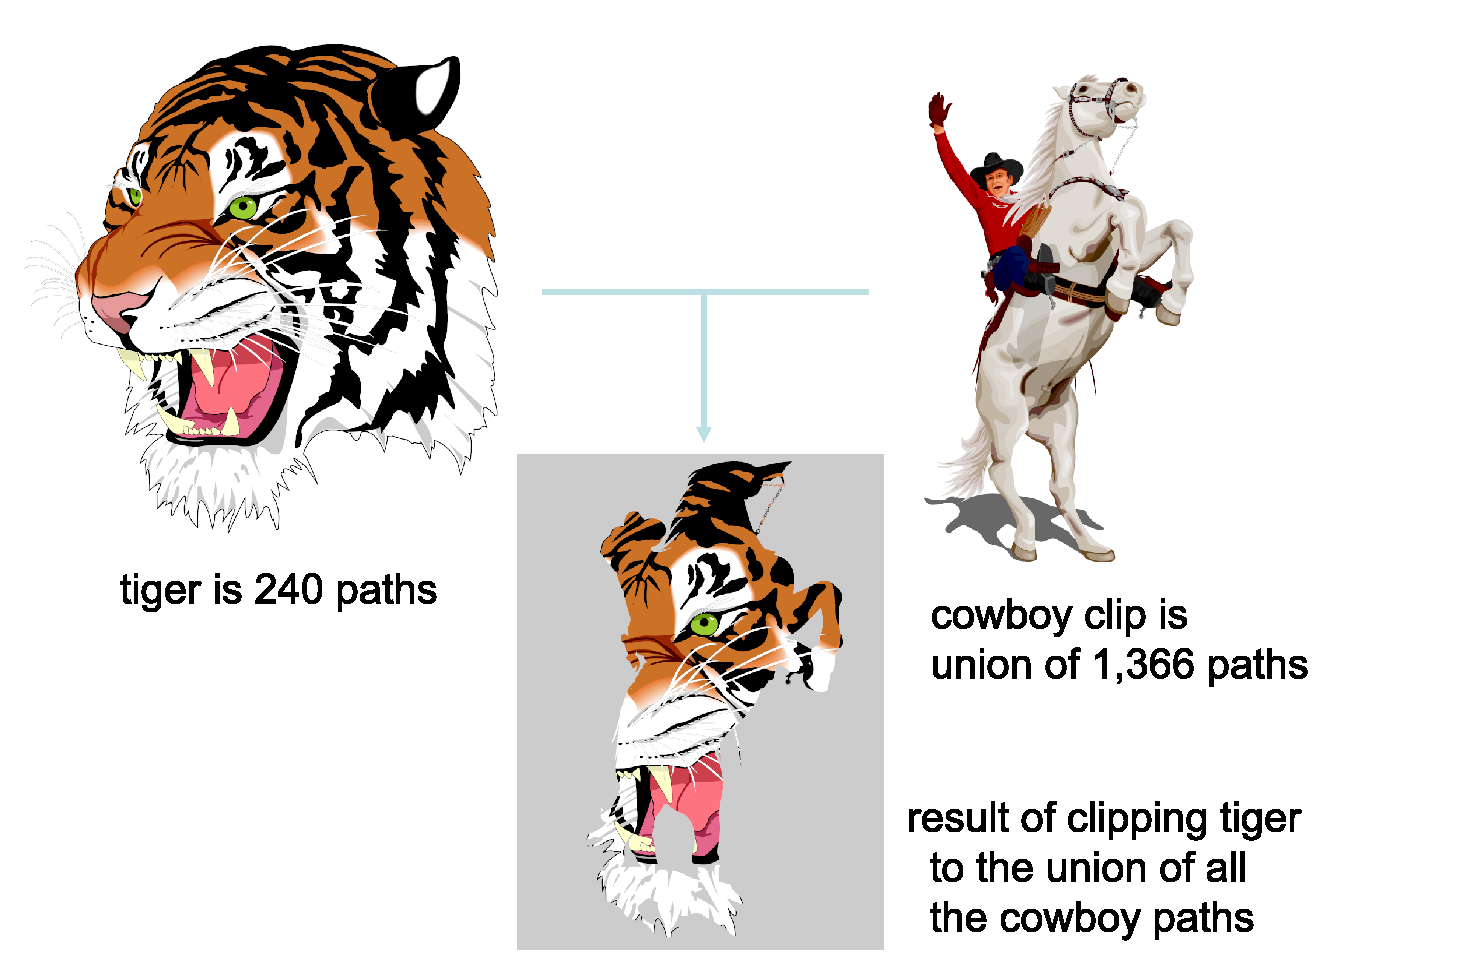
\includegraphics[width=\columnwidth]{clip_example.eps}}
  \center{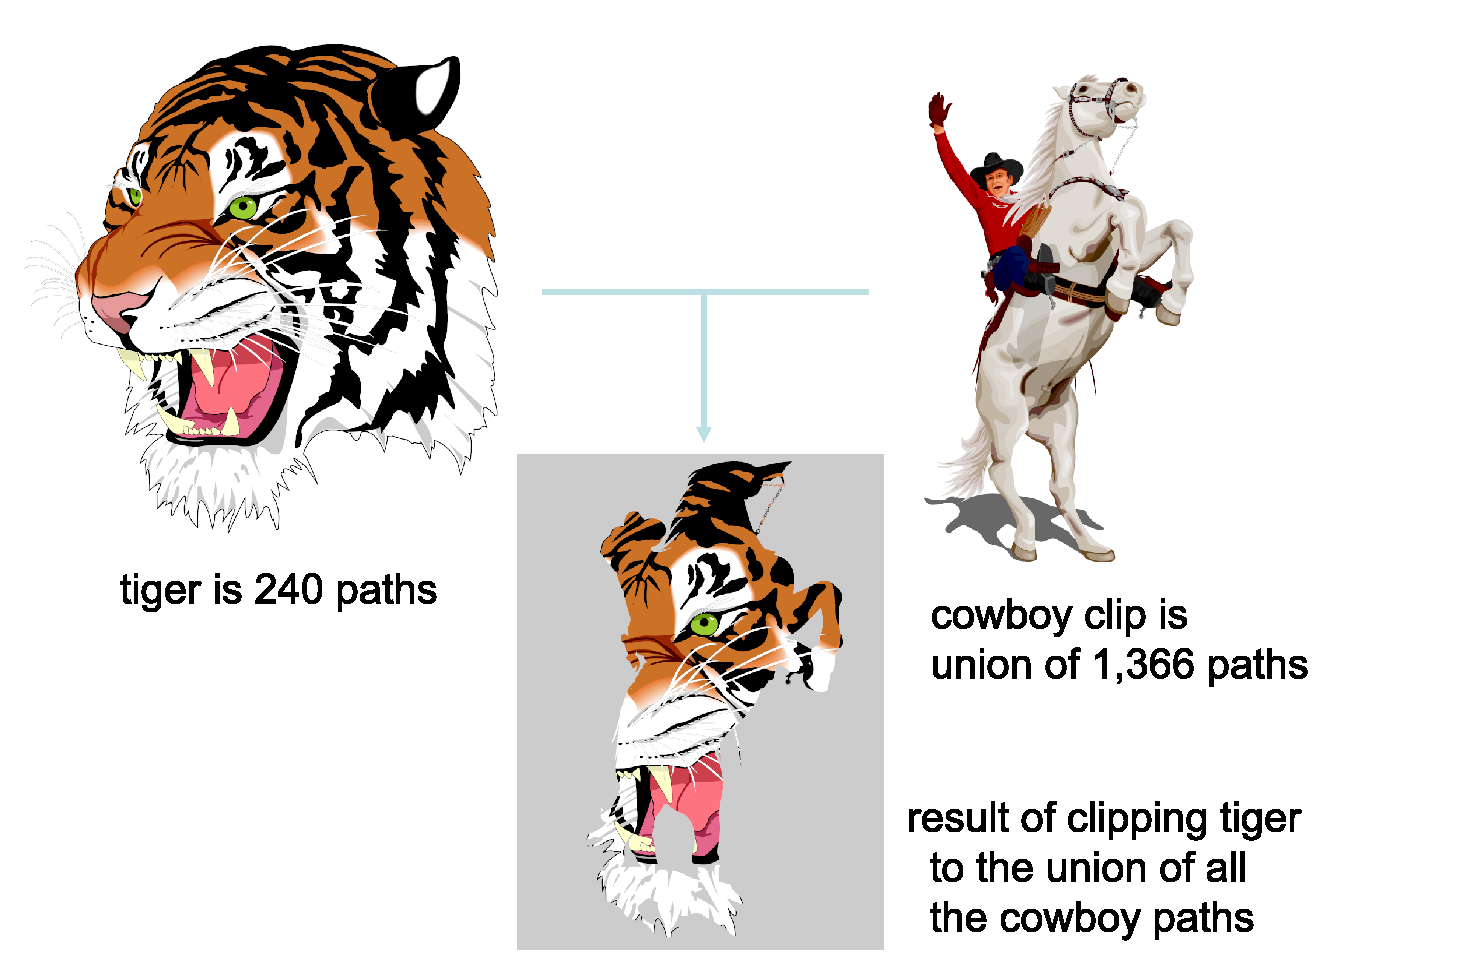
\includegraphics[width=3.6in]{clip_example.eps}}
  \caption{\label{fig:clip-example} Complex clipping scenario.
  Our approach: 8.69ms @ 1000x1000x16.  Cairo:  909ms @ 1000x1000.
  System: Core i7 + GeForce 560M GPU.}
\end{figure}

\subsection{Clipping to Arbitrary Paths}

All major path rendering standards support clipping a {\em draw}
path to the filled region of a {\em clip} path.
Our two-step ``stencil, then cover'' approach readily supports clipping
to arbitrary paths.  We briefly describe the process assuming an 8-bit
stencil buffer, initially cleared to zero:
%\vspace{-3pt}
\begin{enumerate}
  \item Stencil the clip path into the stencil buffer with a ``stencil
  fill'' operation.
  \item Perform a ``cover fill'' operation to coalesce the samples
  matching the fill rule so that the most-significant stencil bit is
  set and all the lower bits are cleared.  For example, if a sample's stencil
  value is non-zero, replace the stencil value with 0x80.
  This step updates only the stencil buffer (disable any color writes).
  \item Stencil the draw path into the stencil buffer with a ``stencil
  fill'' operation, but (a) modify only the bottom 7 bits of the stencil
  buffer, and (b) discard any rasterized samples without the topmost
  bit of the stencil buffer set.
  \item Perform a shaded ``cover'' operation on the draw path.  Update any
  color sample whose stencil value's bottom 7 bits are non-zero and
  zero the bottom 7 bits of the sample's stencil value.  Write shaded
  color samples during this step; due to the stencil configuration, only
  samples within both the clip and draw paths get shaded and updated.
  \item Finally to undo the clip path's stencil manipulation from step
  1, perform a ``cover'' operation on the clip path to reset the most
  significant stencil bit back to zero.
\end{enumerate}
Many variations on this approach are possible.  For example, steps
3 and 4 can be repeated for each path in a layered group of paths.
This avoids having to re-render the clip path for each and every path
in a group of paths.

Most standards allow nested clipping of paths to other paths.  Clever
manipulation of the stencil bit-planes allows such nested clipping.
Standards such as SVG allow for clipping to the union of an arbitrary
number of paths as shown in Figure \ref{fig:clip-example}.  Again, we can
accomplish this by clever use of stencil bit-planes and re-coalescing
coverage from different clip paths.
%  Conventional path clipping is the
%intersection of one path with another, but we can use the stencil buffer
%to compute the union, complement, or intersection of paths too.

\subsection{Painting}

What path rendering standards often call ``painting'' a filled or stroked
path is called shading in 3D graphics.  Our goal is to allow the full
generality of GPU-based programmable shading to be exposed when painting
paths.

During the cover step where a conservative bounding box or convex hull
is rendered to cover fully the stenciling of the path, the application
can configure arbitrary OpenGL shading.  This could be fixed-function
shading, assembly-level shaders, or shaders written in a high-level
language such as Cg or GLSL.

In conventional path rendering systems, linear and radial gradients are
a common form of paint for paths.  We note how straightforward radial
gradient paint can be implemented, including mipmapped filtering of the
lookup table accesses, with the following Cg shader:
%\vspace{-3pt}
\begin{lstlisting}
void radialFocalGradient(float3 str : TEXCOORD0.CENTROID,
                         float4 c   : COLOR.CENTROID,
                     out float4 color   : COLOR,
                 uniform sampler1D ramp : TEXUNIT0)
{
  color = c*tex1D(ramp, length(str.xy) + str.z);
}
\end{lstlisting}
%\vspace{-1em}
The texture coordinates needed for this shader can be generated as a
linear function of the path-space coordinate system.
Painting need not be limited to conventional types of path rendering
paint.  Arbitrary fragment shader processing can be performed during
the cover step (see Figure \ref{fig:bumpmap}).

\begin{figure}[tb]
  %\center{
\includegraphics[width=\columnwidth]{bumpmap.eps}}
  \center{
\includegraphics[width=3.3in]{bumpmap.eps}}
  \caption{\label{fig:bumpmap} Bump map shader applied to path rendered
  text, rendered from to different light positions, shown in yellow.}
\end{figure}

\subsection{Blending and Blend Modes}

OpenGL blending is sufficient for most path rendering where the
default path compositing operation is the ``over'' blend mode, assuming
pre-multiplied alpha.  Color writes during our cover step apply the
currently configured OpenGL blend state.
Modern GPUs also have efficient first-class support for blending in the
widely-used sRGB device color space.

%\subsubsection{sRGB Color Space}
%
%Modern GPUs have first-class support for blending in the sRGB color space.
%Such blending, while recognized as more correct for the broad variety of
%sRGB display devices, has been too expensive to justify for CPU-based
%path renderers.  With our approach, sRGB blending is easily configured
%with OpenGL and fast.

Sophisticated path rendering systems have additional blend modes
\cite{SVG-Compositing-Spec} beyond the standard Porter-Duff compositing
algebra \shortcite{Porter:1984:CDI:800031.808606}.  Digital artists are
familiar with these modes with names such as {\em ColorDodge}, {\em HardLight}, etc.
However GPU blending does not support these blend modes because they are
rare, complex, and not used by 3D graphics.  While some of these blend
modes can be simulated with multiple rendering passes, many of these modes
are impossible to construct from conventional GPU blending operations.

Our ``stencil, then cover'' approach makes it possible to implement
these blend modes despite their lack of direct GPU hardware support.
Normally, GPUs do not reliably support reading-as-a-texture a framebuffer
currently being rendered.  However a recent OpenGL extension called
{\tt NV\_texture\_barrier} \cite{TextureBarrier} provides a reliable memory
barrier under restrictive conditions.  A fragment shader must ensure
there is a single read and write for any particular pixel done from that
pixel's fragment shader instance.

The ``stencil, then cover'' approach provides precisely such a
``no double blending'' guarantee.  So by preceding each cover operation
(whether fill or stroke) with an OpenGL {\tt glTextureBarrierNV}  command and
reading the pixel's color value as a fetch to the framebuffer bound as
a texture, reliable programmable blending with the fragment shader is
possible.



%
\section{Introduction}
\label{sec:api}

Our SIGGRAPH Asia paper {\em GPU-accelerated Path Rendering} \cite{KilgardBolz2012}
describes a system for accelerating vector graphics on GPUs. NVIDIA has
implemented the system and has been shipping the functionality for its GeForce and Quadro GPUs since the summer of 2011.
We refer the reader to that paper for the motivation and technical underpinning
of the {\tt NV\_path\_rendering} \cite{NVpr} OpenGL extension.  In particular, that
paper explains our ``Stencil, then Cover'' (StC) approach to filling and stenciling paths.

In this annex to the forementioned paper we explain the programming interface in
more detail.  The intended audience for this annex is developers
evaluating and learning to program {\tt NV\_path\_rendering}.  You should
be familiar with the OpenGL \cite{OpenGLspec} programming interface.
Familiarity with path rendering standards such as PostScript or SVG is helpful.

Figure~\ref{fig:pipelines} shows how our new path pipeline co-exists
with the existing pipelines in OpenGL for pixel and vertex processing.
Your application can {\em mix} traditional OpenGL usage with path rendering.

\section{Path Object Specification}

Before an application can render paths, it must create a path object
corresponding to each path.  A path object is a container for the sequence
of path commands and corresponding coordinates for the path.  Additionally, each path
object maintains per-object parameters (see Section~\ref{api:parameters})
and the ``baked'' GPU-resident state needed to stencil and cover the path
object.  Like other types of objects in OpenGL, path objects are named
by 32-bit unsigned integers.  Names of path objects can be generated,
tested for existence, and deleted respectively with {\tt glGenPathsNV}, {\tt glIsPathNV},
and {\tt glDeletePathsNV} commands---matching the mechanism OpenGL uses for texture,
buffer, and display list objects.
\begin{table*}[htb]
\begin{center}
{\small
\begin{tabular}{|l|c|c|c|c|}
\hline
                   & {\bf Relative} & {\bf Number of scalar}   & {\bf Character} & \\
{\bf Path command} & {\bf version}  & {\bf coordinates} & {\bf alias} & {\bf Origin} \\
\hline \hline
{\tt GL\_MOVE\_TO\_NV} & \tickYes & 2 & M/m & {\em all} \\
\hline
{\tt GL\_LINE\_TO\_NV} & \tickYes & 2 & L/l & {\em all} \\
{\tt GL\_HORIZONTAL\_LINE\_NV} & \tickYes & 1 & H/h & SVG \\
{\tt GL\_VERTICAL\_LINE\_NV} & \tickYes & 1 & V/v & SVG \\
\hline
{\tt GL\_QUADRATIC\_CURVE\_TO\_NV} & \tickYes & 4 & Q/q & SVG \\
{\tt GL\_CUBIC\_CURVE\_TO\_NV} & \tickYes & 6 & C/c & {\em all} \\
{\tt GL\_SMOOTH\_QUADRATIC\_CURVE\_TO\_NV} & \tickYes & 2 & T/t & SVG \\
{\tt GL\_SMOOTH\_CUBIC\_CURVE\_TO\_NV} & \tickYes & 4 & S/s & SVG \\
\hline
{\tt GL\_SMALL\_CCW\_ARC\_TO\_NV} & \tickYes & 5 & - & OpenVG \\
{\tt GL\_SMALL\_CW\_ARC\_TO\_NV} & \tickYes & 5 & - & OpenVG \\
{\tt GL\_LARGE\_CCW\_ARC\_TO\_NV} & \tickYes & 5 & - & OpenVG \\
{\tt GL\_LARGE\_CW\_ARC\_TO\_NV} & \tickYes & 5 & - & OpenVG \\
\hline
{\tt GL\_ARC\_TO\_NV} & \tickYes & 7 & A/a & SVG \\
\hline
{\tt GL\_CIRCULAR\_CCW\_ARC\_TO\_NV} & \tickNo & 5 & - & PostScript \\
{\tt GL\_CIRCULAR\_CW\_ARC\_TO\_NV} & \tickNo & 5 & - & PostScript \\
{\tt GL\_CIRCULAR\_TANGENT\_ARC\_TO\_NV} & \tickNo & 5 & - & PostScript \\
\hline
{\tt GL\_RECT\_NV} & \tickNo & 4 & - & PDF \\
{\tt GL\_DUP\_FIRST\_CUBIC\_CURVE\_TO\_NV} & \tickNo & 4 & - & PDF \\
{\tt GL\_DUP\_LAST\_CUBIC\_CURVE\_TO\_NV} & \tickNo & 4 & - & PDF \\
\hline
{\tt GL\_RESTART\_PATH\_NV} & \tickNo & 0 & - & PostScript \\
{\tt GL\_CLOSE\_PATH\_NV} & \tickNo & 0 & - & {\em all} \\
\hline
\end{tabular}
}
\caption{Path commands supported by {\tt NV\_path\_rendering}.  The character alias
column provides an ASCII alias for the absolute/relative version of
token.  The ``all'' for origin means the path command is common to all path rendering standards.
}
\label{tab:commands}
\end{center}
\end{table*}

\subsection{Path Segment Commands}

The path commands supported by {\tt NV\_path\_rendering} are the union
of path commands from all major path rendering standards.  We designed
{\tt NV\_path\_rendering} to be a low-level interface upon which all
major path rendering standards can be hosted.  Eliminating any semantic
friction between the path commands of various standards and our interface
is important to us.

For example, PostScript \cite{PLRM} provides three commands ({\tt arc}, {\tt arcn},
and {\tt arct}) for specifying circular arc segments.  While standards
developed after PostScript sought to generalize circular arc segments to
an elliptical form, our interface supports circular arc commands to match
PostScript's parameterization.  So rather than require an application
to convert such PostScript circular paths into some alternate form,
the circular arc commands are handled with semantics exactly matching
PostScript.  Likewise, OpenVG \cite{OpenVG-Spec} has a four elliptical arc segment commands,
each expecting five coordinate values; whereas SVG has a single elliptical
arc segment command with five continuous coordinate values and two
Boolean coordinates.

For line segments, the general line segment command takes an $(x,y)$
control point---but horizontal and vertical line segments take a single
horizontal or vertical coordinate respectively.

For B\'{e}zier curve segments, commands exist for smooth B\'{e}zier
segments, matching up with the prior command's segment to provide C1
continuity.

Where appropriate, we provide relative and absolute versions of all
path commands.  With relative commands, path coordinates indicating a
position are relative to the end point of the prior path segment.

In addition to eliminating the semantic gap between other path standards
and our interface, we note that paths can be represented with fewer
path coordinates when the variety of available path commands is broad.
Also, editing of the sequence of path commands and coordinates
is straightforward when each standard's path command vocabulary is
supported directly.  Table~\ref{tab:commands} organizes the supported
path commands.

Path objects are specified in four ways:
\begin{enumerate}
  \item Explicitly, from a sequence of path commands and their
  corresponding path coordinates.
  \item From a string conforming to a standard grammar for specifying
  a paths.  Both PostScript and SVG have standard grammars for paths---and
  we support both.
  \item From a Unicode character point of an outline font.  A font
  can be specified with a system name (such as Helvetica or Arial),
  an outline font filename, or a built-in font.
  \item Derived from one or more existing path objects.  The new path
  may be the result of an arbitrary projective transform of an existing
  path, or the linear weighting of existing paths with matching command
  sequences.
\end{enumerate}

\begin{figure}[t]
  %\center{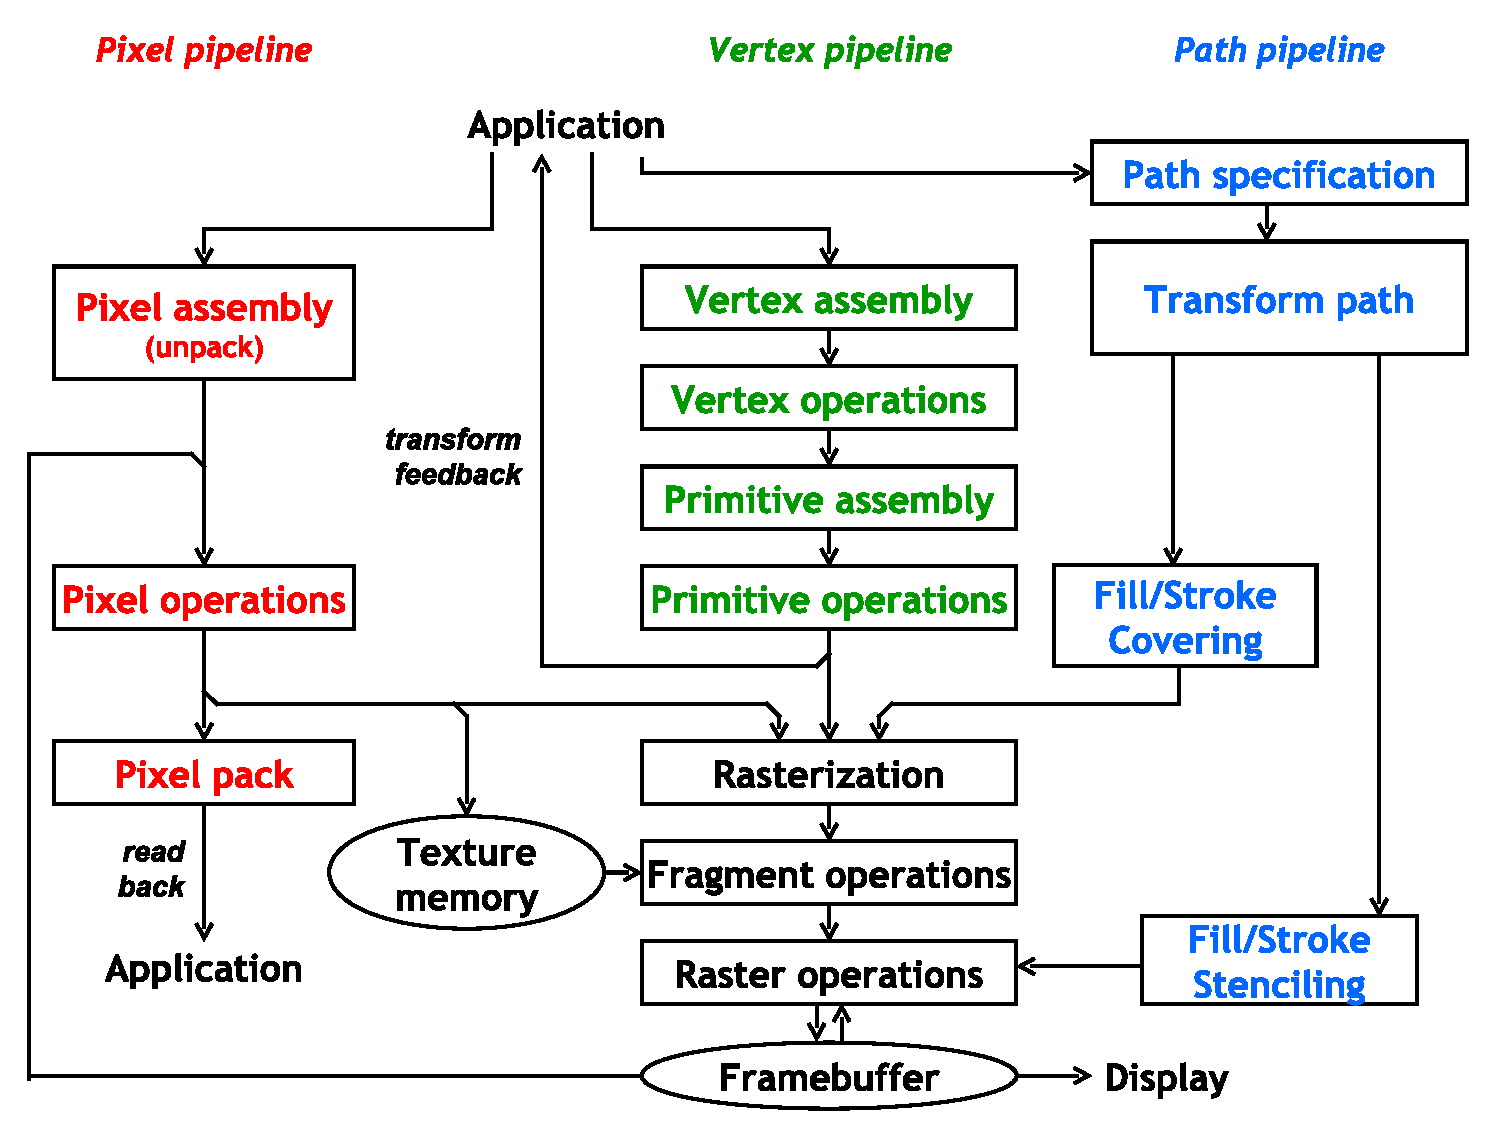
\includegraphics[width=\columnwidth]{pipelines.eps}}
  \center{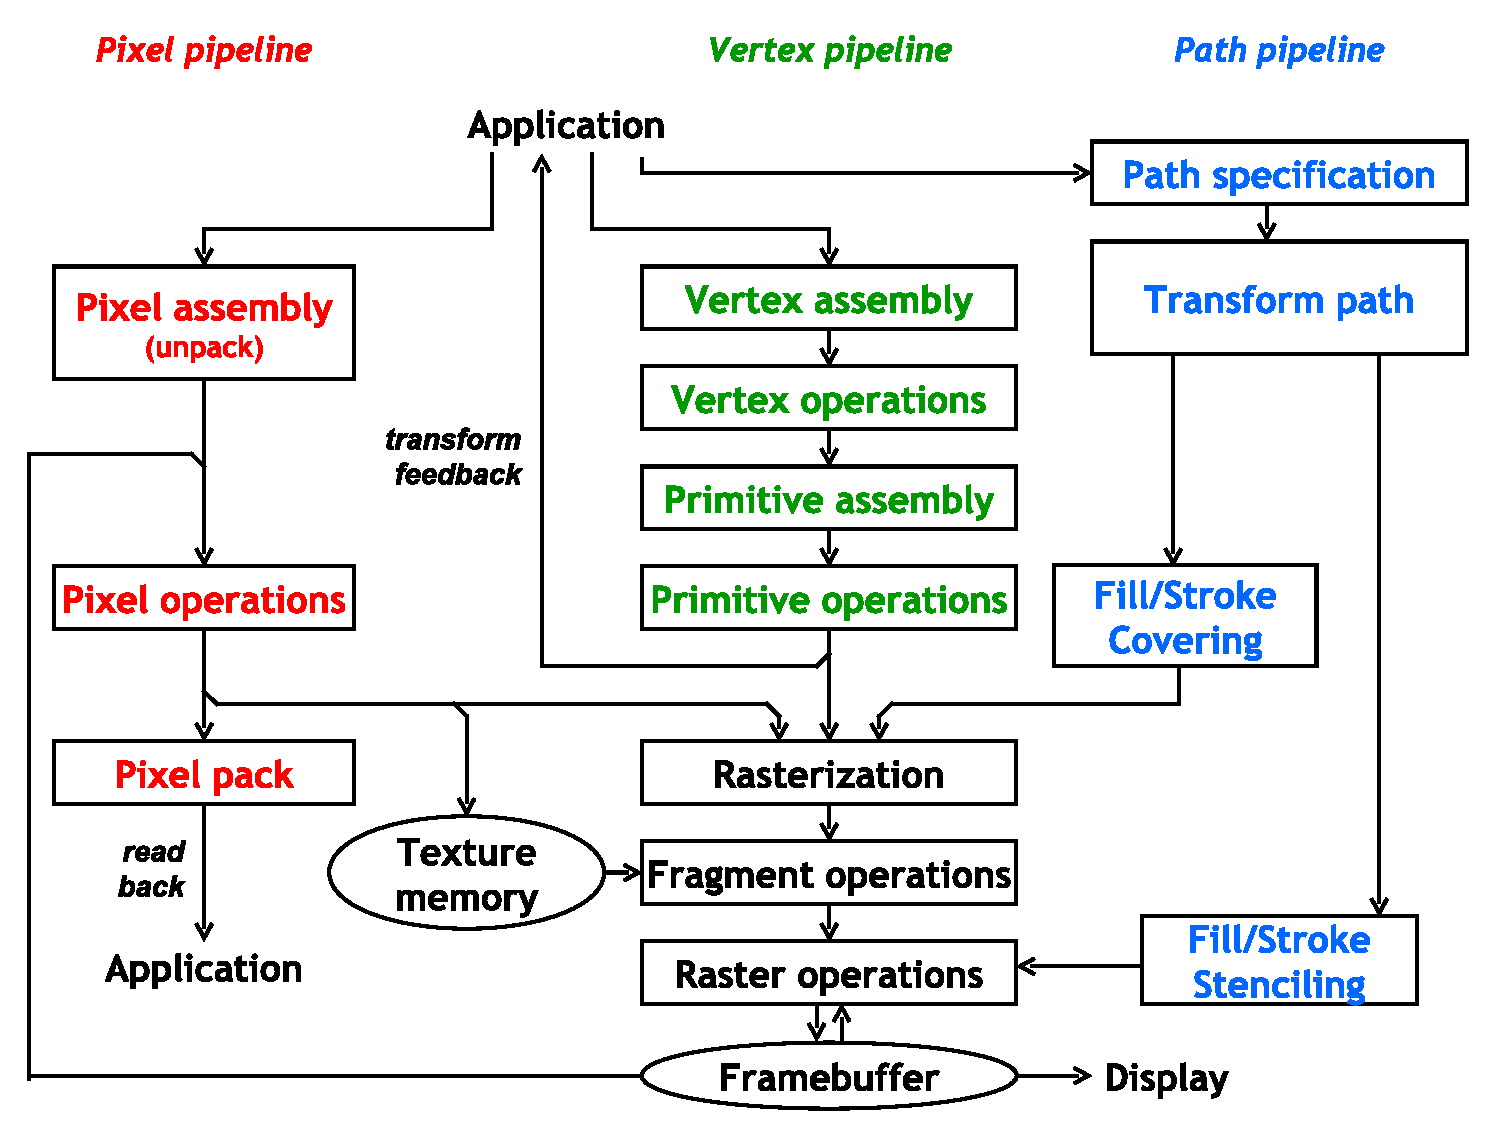
\includegraphics[width=\columnwidth]{pipelines.eps}}
  \caption{\label{fig:pipelines} High-level data flow of OpenGL showing
  pixel, vertex, and new path pipelines.}
\end{figure}

\subsection{Explicit Path Specification}

The command
\begin{lstlisting}
  void glPathCommandsNV(GLuint path,
                        GLsizei numCmds,
                        const GLubyte *cmds,
                        GLsizei numCoords,
                        GLenum coordType,
                        const void *coords);
\end{lstlisting}
specifies a new path object named {\em path} where {\em numCmds} indicates
the number of path commands, read from the array {\em commands}, with
which to initialize that path's command sequence.  These path commands
reference coordinates read sequentially from the {\em coords} array.
The type of the coordinates read from the {\em coords} array is determined
by the {\em coordType} parameter which must be one of {\tt GL\_BYTE}, {\tt
GL\_UNSIGNED\_BYTE}, {\tt GL\_SHORT}, {\tt GL\_UNSIGNED\_SHORT}, or {\tt GL\_FLOAT}.
Coordinates supplied in more compact data types allows paths to be stored
more efficiently.

The {\em numCmds} elements of the {\em cmds} array must be tokens (or
character aliases) from Table~\ref{tab:commands}.  The command sequence
matches the element order of the {\em cmds} array.  Each command
references a number of coordinates specified by the ``Number of scalar
coordinates'' column of Table~\ref{tab:commands}, starting with the first
(zero) element of the coords array and advancing by the coordinate count
for each command.

The following code fragment creates path object 42 containing the contours
of a five-point star and heart:
\begin{lstlisting}
  static const GLubyte pathCommands[10] =
    { GL_MOVE_TO_NV, GL_LINE_TO_NV,
      GL_LINE_TO_NV, GL_LINE_TO_NV,
      GL_LINE_TO_NV, GL_CLOSE_PATH_NV,
      'M', 'C', 'C', 'Z' };  // character aliases
  static const GLshort pathCoords[12][2] =
    { {100,180}, {40,10}, {190,120}, {10,120}, {160,10},
      {300,300}, {100,400}, {100,200}, {300,100},
      {500,200}, {500,400}, {300,300} };
  GLuint pathObj = 42;
  glPathCommandsNV(pathObj, 10, pathCommands,
    24, GL_SHORT, pathCoords);
\end{lstlisting}
The example demonstrates how tokens or character aliases can be used
interchangeably to specify a path.

\subsection{Grammars for Path Specification}

The command 
\begin{lstlisting}
  glPathStringNV(GLuint path, GLenum format,
                 GLsizei length, const void *pathString);
\end{lstlisting}
specifies a new path object named {\em path} where format must be either
{\tt GL\_PATH\_FORMAT\_SVG\_NV} or {\tt GL\_PATH\_FORMAT\_PS\_NV}, in which case the
{\em length} and {\em pathString} are interpreted respectively according to
SVG's grammar\footnote{The Backus-Naur Form (BNF) description of the SVG path grammar is found here \url{http://www.w3.org/TR/SVG/paths.html\#PathDataBNF}}
for paths or PostScript's sub-grammar for user paths.
This code fragment is functionally identical to the prior explicit path
specification example but uses an SVG path string:
\begin{lstlisting}
  const char *svgPathString =
    // star
    "M100,180 L40,10 L190,120 L10,120 L160,10 z"
    // heart
    "M300 300 "
    "C100 400,100 200,300 100,500 200,500 400,300 300Z";
  glPathStringNV(pathObj, GL_PATH_FORMAT_SVG_NV,
    (GLsizei)strlen(svgPathString), svgPathString);
\end{lstlisting}
Creating paths from strings has proven very convenient and avoids having
each application re-implement standard path grammar parsers.

\subsection{Specifying Paths from Glyphs of a Font}

Text rendering is a first-class feature in every major path rendering
API and standard.  Requiring applications to load outlines of glyphs
is just too common, not to mention arduous and platform-dependent,
so {\tt NV\_path\_rendering} provides a mechanism for applications to
create path objects from glyphs---including contiguous ranges of glyphs
indexed by their Unicode character points.

Two commands {\tt glPathGlyphRangeNV} and {\tt glPathGlyphsNV} create a sequence of path
objects given a font and a range or sequence of Unicode character points
for the font.  The font can be specified using a system font name (such as
``Arial'' or ``Helvetica'' with a file name for a file in a standard font
file format such as TrueType, or a built-in font name (such as ``Sans,''
``Serif,'' or ``Mono'') that is guaranteed to be available on every {\tt
NV\_path\_rendering} implementation, regardless of platform.

Once these path objects are populated, these glyph path objects can be
stenciled and covered, whether filled or stroked, just like any other
path object.

The {\tt glPathGlyphRangeNV} and {\tt glPathGlyphsNV} commands will only
create a path object for a given path name if that path object name
does \underline{not} already correspond to an existing path object.
This behavior is designed to populate path object ranges with glyph
outlines consistent with the {\tt font-family} property of CSS 2.1
\cite{CSS-Spec}.  An application can load a sequence of fonts for a
given range of path objects repeatedly knowing this will resolve to some
supported set of font glyphs eventually.

The {\tt glPathGlyphRangeNV} command has the following prototype:
\begin{lstlisting}
  void glPathGlyphRangeNV(GLuint firstPathName,
                          GLenum fontTarget,
                          GLconst void *fontName,
                          GLbitfield fontStyle,
                          GLuint firstGlyph,
                          GLsizei numGlyphs,
                          GLenum handleMissingGlyphs,
                          GLuint pathParameterTemplate,
                          GLfloat emScale);
\end{lstlisting}
The {\em emScale} parameter allows fonts of different formats to be loaded
with a consistent number of path units per em (a typographic measure of
glyph scale).\footnote{TrueType fonts user 2048 units for their em scale convention; PostScript fonts use 1000.  As most fonts today are based on TrueType conventions, using 2048 is a natural choice.}  Path coordinates and glyph metrics are scaled to match
the specified {\em emScale}.  To ensure all path objects in a range of glyphs
have a consistent set of path parameters, the {\em pathParameterTemplate} path
object names a path object from which the new glyph path objects should
copy their parameters.

This example shows how a range of path objects for sans serif fonts for
the Latin-1 character range can be populated:
\begin{lstlisting}
  // Constants
  const GLint numChars = 256;   // ISO/IEC 8859-1
                                // 8-bit range
  const GLfloat emScale = 2048; // TrueType path
                                // units per em
  
  // Create empty path object for use as parameter template
  GLuint pathTemplate = ~0;  // Biggest path name
  glPathCommandsNV(pathTemplate,
    0, NULL, 0, GL_FLOAT, NULL);
  glPathParameterfNV(pathTemplate,
    GL_PATH_STROKE_WIDTH_NV, emScale*0.1f);
  glPathParameteriNV(pathTemplate,
    GL_PATH_JOIN_STYLE_NV, GL_MITER_TRUNCATE_NV);
  glPathParameterfNV(pathTemplate,
    GL_PATH_MITER_LIMIT_NV, 1.0);
  // Create path object range for Latin-1 character codes
  GLuint glyphBase = glGenPathsNV(numChars);
  // Typeface names in priority order 
  struct {
    GLenum fontTarget;
    const char *name;
  } font[] = {
    { GL_SYSTEM_FONT_NAME_NV,   "Liberation Sans" },
    { GL_SYSTEM_FONT_NAME_NV,   "Verdana" },
    { GL_SYSTEM_FONT_NAME_NV,   "Arial" },
    // Final standard font provides guaranteed supported
    { GL_STANDARD_FONT_NAME_NV, "Sans" }
  };
  const int numFonts = sizeof(font)/sizeof(font[0]);
  for (int i=0; i< numFonts; i++) {  // For each font
    glPathGlyphRangeNV(glyphBase, 
      font[i].fontTarget, font[i].name, GL_BOLD_BIT_NV,
      0, numChars, GL_USE_MISSING_GLYPH_NV,
      pathTemplate, emScale);
  }
\end{lstlisting}
Path objects loaded from glyphs also have associated glyph and font
metrics loaded corresponding to their character point.  These metrics
and spacing information are discussed in Section~\ref{api:text}.

\subsection{Copied, Weighted, and Transformed Paths}

Additional commands for specifying path objects work by generating a new
path object from one or more existing path objects.  The {\tt glCopyPathNV}
command is the simplest and simply copies the state of a named existing
path object to another path object name.  Path parameters and glyph
metrics are copied by {\tt glCopyPathNV}.

The {\tt glInterpolatePathsNV} command takes two (source) path object names
and a weighting factor and creates a new (destination) path object
that is the linear interpolation based on the weighting factor of the
two source paths.  The {\tt glWeightPathsNV} command generalizes the {\tt
glInterpolatePathsNV} to linear combination of a specified number of source
path objects and corresponding weighting factors.  All the path objects
involved in interpolating or weighting must have identical path command
sequences and contain no circular or elliptical arc segment commands.
The destination path object's parameters are copied from the first
destination path object; glyph metrics are all set invalid (to -1).

The {\tt glTransformPathNV} command take a source path object name and
generates a new named destination path object corresponding to the
destination path object transformed by an affine linear transform.
Path commands such as horizontal or vertical lines or circular arcs may
be promoted to a more general path command form as required to perform
the transformation.  Relative commands are converted to absolute commands,
transformed, and then converted back to relative commands.

If the destination path object name refers to an existing path object,
that path object is replaced (implicitly deleting the old object) with the
new path object.  The destination name may be one of the source names.

Assuming the implementation performs a lazy copy of path commands and
coordinates, {\tt glCopyPathNV} allows efficient rendering of a path with
different stroking parameters.  {\tt glInterpolatePathsNV} can help implement
Flash's Shape Morph functionality and OpenVG's {\tt vgInterpolatePath}
command.  {\tt glTransformPathNV} can help implement SVG 1.2's non-scaling
stroke functionality and OpenVG's {\tt vgTransformPath}. 

\section{Path Parameters}
\label{api:parameters}

Every path object has state in addition to its sequence of path commands
and coordinates.

\subsection{Settable Parameters}

The {\tt glPathParameteriNV}, {\tt glPathParameterfNV}, {\tt glPathParameterivNV},
and {\tt glPathParameterfvNV} commands respectively set path parameters of
a specified path object given integer or float data supplied by a scalar
parameter or vector array.

Table~\ref{tab:parameters} summarizes the settable parameters.  Many
parameters deal with embellishments to stroking such as the stroke width,
join style, miter limit, end caps, and dash caps.
\begin{table}[htb]
\begin{center}
{\small
\begin{tabular}{|l|l|l|}
\hline
{\bf Name} & {\bf Type} & {\bf Initial value} \\
\hline
\hline
{\tt GL\_PATH\_STROKE\_WIDTH\_NV} & $\Re+$ & 1.0 \\
\hline
{\tt GL\_PATH\_JOIN\_STYLE\_NV} & 4-valued & {\tt GL\_MITER\_REVERT\_NV} \\
{\tt GL\_PATH\_MITER\_LIMIT\_NV} & $\Re+$ & 4 \\
\hline
{\tt GL\_PATH\_INITIAL\_END\_CAP\_NV} & 4-valued & {\tt GL\_FLAT} \\
{\tt GL\_PATH\_TERMINAL\_END\_CAP\_NV} & 4-valued & {\tt GL\_FLAT} \\
\hline
{\tt GL\_PATH\_INITIAL\_DASH\_CAP\_NV} & 4-valued & {\tt GL\_FLAT} \\
{\tt GL\_PATH\_TERMINAL\_DASH\_CAP\_NV} & 4-valued & {\tt GL\_FLAT} \\
{\tt GL\_PATH\_DASH\_OFFSET\_NV} & $\Re$ & 0.0 \\
{\tt GL\_PATH\_DASH\_OFFSET\_RESET\_NV} & 2-valued & {\tt GL\_MOVE\_TO\_CONTINUES\_NV} \\
\hline
{\tt GL\_PATH\_CLIENT\_LENGTH\_NV} & $\Re+$ & 0.0 \\
\hline
{\tt GL\_PATH\_FILL\_MODE\_NV} & 4-valued & {\tt GL\_COUNT\_UP\_NV} \\
{\tt GL\_PATH\_FILL\_MASK\_NV} & mask & all 1's \\
{\tt GL\_PATH\_FILL\_COVER\_MODE\_NV} & 3-valued & {\tt GL\_CONVEX\_HULL\_NV} \\
\hline
{\tt GL\_PATH\_STROKE\_COVER\_MODE\_NV} & 3-valued & {\tt GL\_CONVEX\_HULL\_NV} \\
{\tt GL\_PATH\_STROKE\_MASK\_NV} & mask & all 1's \\
\hline
\end{tabular}
}
\end{center}
\caption{Settable path object parameters.}
\label{tab:parameters}
\end{table}

\subsection{Dashing State}

Dashing is an embellishment to stroking where a repeated pattern of
enabled stroking and gaps in stroking is applied during stroking.
The conventional {\tt glPathParameteriNV}, etc. commands are ill-suited to
setting a variable number of dash offsets.

Instead parameters to control the dash pattern of a stroked path are
specified by the command
\begin{lstlisting}
  void glPathDashArrayNV(GLuint path,
                         GLsizei dashCount,
                         const GLfloat *dashArray);
\end{lstlisting}
where {\em path} is the name of an existing path object.  A {\em
dashCount} of zero indicates the path object is not dashed; in this case,
the {\em dashArray} is not accessed.  Otherwise, {\em dashCount} provides
a count of how many float values to read from the {\em dashArray} array.
The values provide an on/off pattern for dashing.  If the dash pattern is [3,1,3,2],
this indicates the dashing will repeat being on for 3 path-space units, off for 1
unit, on for 3 units, off for 2 units, etc.\footnote{An odd number of values ``doubles''
the specified pattern to make an even on/off pattern.}

\subsection{Computed Parameters and Querying State}

All settable path object state is able to be queried; this
includes settable parameters with {\tt glGetPathParameterivNV} and {\tt
glGetPathParameterfvNV}, the dashing array with {\tt glGetPathDashArrayNV},
the path command array with {\tt glGetPathCommandsNV}, and path coordinate
array with {\tt glGetPathCoordsNV}.  Additionally, computed parameters for
each path object can be queried; see Table~\ref{tab:computed}.
\begin{table}[htb]
\begin{center}
{\small
\begin{tabular}{|l|l|}
\hline
{\bf Name} & {\bf Type} \\
\hline
\hline
{\tt GL\_PATH\_COMMAND\_COUNT\_NV} & N \\
{\tt GL\_PATH\_COORD\_COUNT\_NV} & N \\
\hline
{\tt GL\_PATH\_COMPUTED\_LENGTH\_NV} & $\Re+$ \\
\hline
{\tt GL\_PATH\_OBJECT\_BOUNDING\_BOX\_NV} & $4\times\Re$ \\
{\tt GL\_PATH\_FILL\_BOUNDING\_BOX\_NV} & $4\times\Re$ \\
{\tt GL\_PATH\_STROKE\_BOUNDING\_BOX\_NV} & $4\times\Re$ \\
\hline
\end{tabular}
}
\end{center}
\caption{Computed path object parameters.}
\label{tab:computed}
\end{table}

\subsection{Glyph and Font Metrics}

Path objects created from character points from a font are tagged with
additional read-only glyph metrics.  These metrics are useful for text
layout.  Additionally, every glyph has aggregate per-font metrics for
its corresponding font.  The metrics are obtained directly from the font
except for any scaling based on the {\em emScale}.  The {\tt glGetPathMetricRangeNV}
and {\tt glGetPathMetricsNV} queries return the glyph and per-font metrics for a
range or sequence of path objects respectively.

As shown in Figure~\ref{fig:glyph-metrics}, the glyph metrics provide each
glyph's width and height and $(x,y)$ bearing and advance for both horizontal
and vertical layout.  These metrics are expressed in path space units.
 
\begin{figure}[b]
  \center{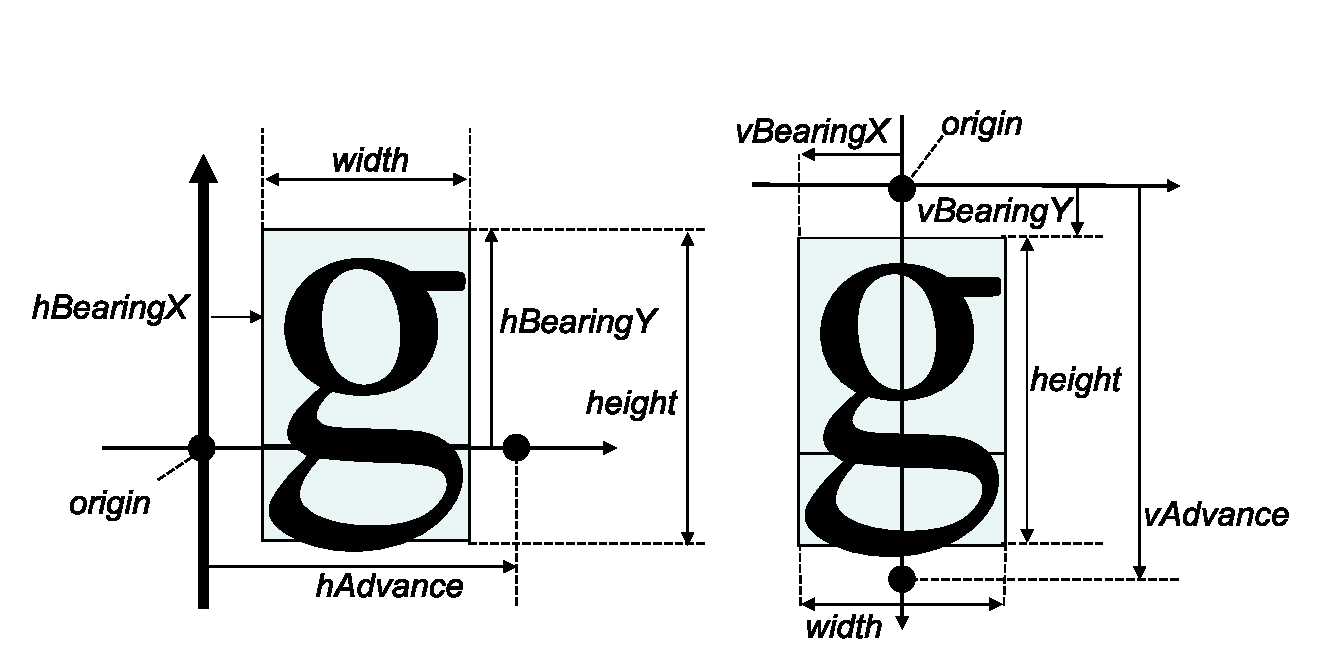
\includegraphics[width=\columnwidth]{glyph_metrics.eps}}
  \caption{\label{fig:glyph-metrics} Glyph metrics.}
\end{figure}

Additional per-font metrics can be queried from any glyph belonging to a
particular font.  These metrics include a bounding box large enough to
contain any glyph in the font, the native number of font units per em,
the font-wide ascender, descender, and height distances, maximum advance
for horizontal and vertical layout, underline position and thickness.

Requested metrics are specified in a bitmask and returned to an
application-provided array of floats.

\section{Rendering Paths via Stencil, then Cover}

Once a path object is created, it can be rendered with the ``stencil,
then cover'' approach.

The mapping from path space to clip space and ultimately window space
is determined by OpenGL's standard modelview, projection, viewport,
and depth range transforms.  An OpenGL programmer familiar with OpenGL's
{\tt glMatrixMode}, {\tt glRotatef}, {\tt glTranslatef}, etc. matrix commands
for transforming 3D geometry uses the same commands to manipulate the
transformations of path objects.

For example, the code below establishes an orthographic path-to-clip-space
to map the $[0..500]\times[0..400]$ region used by the star-and-heart path:
\begin{lstlisting}
  glMatrixLoadIdentityEXT(GL_PROJECTION);
  glMatrixLoadIdentityEXT(GL_MODELVIEW);
  glMatrixOrthoEXT(GL_MODELVIEW, 0, 500, 0, 400, -1, 1);
\end{lstlisting}
This code demonstrates OpenGL's selector-free matrix manipulation
commands introduced by the {\tt EXT\_direct\_state\_access} (DSA) extension \cite{DSA}.

\subsection{Path Rendering in Two Steps}

Now we can render the filled and stroked star-and-heart path.  We assume
the stencil buffer has been initially cleared to zero.

\paragraph{Stencil Step for Filling}

First we stencil the filled region of the star-and-heart path into the
stencil buffer with the {\tt glStencilFillPathNV} command:
\begin{lstlisting}
  glStencilFillPathNV(pathObj, GL_COUNT_UP_NV, 0x1F);
\end{lstlisting}
The winding number of each sample in the framebuffer w.r.t. the
transformed path is added ({\tt GL\_COUNT\_UP}) to the stencil value corresponding
to each rasterized same.   The 0x1F mask indicates that only the five
least significant stencil bits are modified---effectively resulting in
modulo-32 addition.  More typically, this mask will be 0xFF.

Instead of {\tt GL\_COUNT\_UP}, we could also subtract ({\tt GL\_COUNT\_DOWN})
or invert bits ({\tt GL\_INVERT}) by a count equal to each sample's winding
number w.r.t. the transformed path.

\paragraph{Cover Step for Filling}

Second we conservatively cover the previously stenciled filled region
of the star-and heart path.  The shading, stencil testing, and blending
are fully controlled by the application's OpenGL context state during
the cover.  So we first enable stencil testing to discard color samples
with a stencil value of zero (those not in the path as determined by
the prior stencil step); for samples that survive the stencil test,
we want to reset the stencil value to zero and shade the corresponding
sample's color value green.  So:
\begin{lstlisting}
  glEnable(GL_STENCIL_TEST);
  glStencilFunc(GL_NOTEQUAL, 0, 0x1F);
  glStencilOp(GL_KEEP, GL_KEEP, GL_ZERO);
  glColor3f(0,1,0); // green
  glCoverFillPathNV(pathObj, GL_BOUNDING_BOX_NV);
\end{lstlisting}
The result is a green star to the left of a green heart.  A single cover step
updates any particular color sample no more than once; this ensures against
double blending of color samples--as required by path rendering standards.

\paragraph{Stencil Step for Stroking}

Stroking proceeds similarly in two steps; however before rendering, we
configure the path object with desirable path parameters for stroking.
Specify a wider 6.5-unit stroke and the round join style:
\begin{lstlisting}
  glPathParameteriNV(pathObj,
    GL_PATH_JOIN_STYLE_NV, GL_ROUND_NV);
  glPathParameterfNV(pathObj,
    GL_PATH_STROKE_WIDTH_NV, 6.5);
\end{lstlisting}
Now we first stencil the stroked coverage for the heart-and-star path
into the stencil buffer:
\begin{lstlisting}
  glStencilStrokePathNV(pathObj, 0x1, ~0);
\end{lstlisting}
This computes the point containment of every sample in the framebuffer
w.r.t. the stroked path---and if the sample is contained in the path's
stroke, the sample's stencil value is set to 0x1 with a write mask of bit-inverted zero
(writing all stencil bits).

\begin{figure}[tb]
  \center{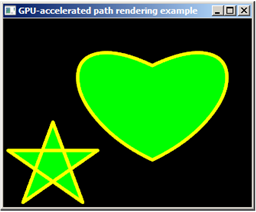
\includegraphics[width=\columnwidth]{star_and_heart.png}}
  \caption{\label{fig:star-and-heart} Filled and stroked path rendering result.}
\end{figure}

\paragraph{Cover Step for Stroking}

Second we conservatively cover the previously stenciled stroked
region of the star-and heart path.  We leave stencil as configured
previously---non-zero values will include the 0x1 value written by the
{\tt glStencilStrokePathNV} command, but we change the color to yellow:
\begin{lstlisting}
  glColor3f(1,1,0); // yellow
  glCoverStrokePathNV(pathObj, CONVEX_HULL);
\end{lstlisting}
The complete rendering result is shown in Figure~\ref{fig:star-and-heart}.

\subsection{Accessible Samples}

The fill and stroke stencil/cover commands {\em conceptually} operate
on all samples in the framebuffer.  Potentially every sample in the
framebuffer could be updated by these commands.  However, the set of {\em
accessible samples} may be restricted the by current OpenGL context state.

Clip planes, polygon stipple, window ownership, scissoring, stencil
testing (on write masked stencil bits during stencil fill/stroke
operations), depth testing, depth bounds testing, and the multisample
mask all limit, when enabled, the accessible samples.

The cover fill/stroke commands further limit the updated samples to the
bounding box or convex hull (depending on the cover mode). 

\subsection{Path Coordinate Generation}

Paths do not have per-vertex attributes such as colors and texture
coordinates that are interpolated over geometric primitives as 3D
geometry does.  Instead varying attributes used by the fragment shader
must be generated as a linear function of the path-space coordinate
system.  The {\tt glPathColorGenNV}, {\tt glPathTexGenNV}, and {\tt glPathFogGenNV}
command generated color, texture coordinate sets, and the fog coordinate
respectively; these loosely mimic OpenGL's fixed-function {\tt glTexGenfvNV},
etc. commands.

For example, to match a common idiom in path rendering standards, the path coordinate
generation supports mapping a path's path space bounding box to a
normalized $[0..1]\times[0..1]$ square.  To apply a 4x3 tile pattern stored in
a repeated 2D texture to the bounding box extents of a covered path, 
configure path texture coordinate generation this way:
\begin{lstlisting}
  const GLfloat coeffs[4] = { 1.0/4, 0,   // s = x/4 + 0
                              1.0/3, 0 }  // t = y/3 + 0
  GLint numCoordinates = 2;  // for s and t
  GLenum texUnit = GL_TEXTURE0;
  glPathTexGenNV(texUnit, GL_PATH_OBJECT_BOUNDING_BOX_NV,
    numCoordinates, coeffs);
  glActiveTexture(texUnit);
  glEnable(GL_TEXTURE_2D);
\end{lstlisting}

\section{Text Handling}
\label{api:text}

\subsection{Instanced Rendering}

Efficient rendering of glyphs is very important for any path rendering
system.  In addition to the ability to create path objects from Unicode
character points of fonts and query glyph metrics for such path objects,
instanced commands for stenciling and covering sequences of path objects
in a single OpenGL command are provided.

{\tt glStencilFillPathInstancedNV} and {\tt glCoverFillPathInstancedNV}
for filling and {\tt glStencilStrokePathInstancedNV} and {\tt
glCoverStrokePathInstancedNV} for stroking accept arrays of path objects
where each path object instance has its own local transformation.

This is intended for rendering spans of characters with corresponding
glyph path objects, but could be used for rendering any sequence of
path objects.  To facilitate text, there is a base path object value to
which each path object offset in the sequence is added.  This allows a
string of ASCII characters to be provided where the base path object
value identifies the base of a range of glyphs specified with {\tt
glPathGlyphRangeNV}.  The array of offsets can even be a UTF-8 or UTF-16
string to facilitate easy rendering of Unicode text.

The instanced cover commands include a special
{\tt GL\_BOUNDING\_BOX\_-OF\_BOUNDING\_BOXES} cover mode where the bounding boxes
of each locally transformed path object's cover geometry is combined
({\em unioned}) into a single bounding box.

These instanced commands give the OpenGL implementation the freedom to
reorder the geometry sets used during the instanced stencil step for
better efficiency in the GPU.  

\subsection{Spacing and Kerning}

Good aesthetics and legibility for horizontal spans of text generally
involves appropriate spacing for the glyphs.  When this spacing depends
on which pairs of glyphs are mutually adjacent, this is called kerning.
We provide a {\tt glGetPathSpacingNV} query that accepts a sequence of path objects
(in the same way the instanced stencil/cover commands do) and returns an
array of translations corresponding to the kerned spacing of the glyphs.

The returned array of translations from {\tt glGetPathSpacingNV} is immediately
suitable to pass as the array of translations used for the local
transformation sequence when using the instanced stencil/cover commands.

While applications with complex text layout requirements might judge this
mechanism insufficiently sophisticated, because the mechanism is simple,
cross-platform, and generates kerned glyph translations as expected by
the instanced stencil/cover commands, we anticipate this functionality
will meet the basic text layout needs of many applications.

\section{Geometric Queries}

{\tt NV\_path\_rendering} includes a set of common geometric queries on
paths.  The queries {\tt glIsPointInFillPathNV} and {\tt glIsPointInStrokePathNV} provide
efficient determinations of whether an $(x,y)$ point in a path's local
coordinate system is inside or outside the fill or stroke of the path.
The query {\tt glGetPathLengthNV} provides a means to obtain arc lengths over
specified command sequences for a path.  The query {\tt glPointAlongPathNV}
returns an $(x,y)$ point and $(dx,dy)$ tangent a given arc length into a
path's command sequence.

These queries are intended to be compatible with queries supported by OpenVG.

The crucial rationale for these queries is they are consistent with
our implementation's internal computations for being inside/outside the
path's stroke or fill and arc length computations (such as for dashing).

\section{Antialiasing}

Applications are expected to render into multisample framebuffers to achieve
acceptable antialiasing quality.  Use existing APIs to allocate multisample
framebuffer resources.  {\tt NV\_path\_rendering} automatically generates multisample
coverage when the framebuffer supports multisampling.

Applications can also use OpenGL's accumulation buffer mechanism with jittered
rendering to exceed the base multisampling quality available.



\section{Discussion}
\label{sec:discuss}

\subsection{Quality}

Our system's rendering quality is directly tied to how many color and
stencil samples the framebuffer maintains per pixel.  This determines the
quality of our antialiasing.  Our GeForce GPUs support up to 16 samples
per pixel while our Quadro GPUs support 32 and 64 samples per pixel as
well.

At 16 samples per pixel, our rendering quality compares quite favorably
with CPU-based path renderers.  Because our GPUs have 8 bits of sub-pixel
precision, irregular coverage sample positions, and our point containment
determinations are numerically sound, we are well-justified in stating
our quality exceeds what can reasonably be expected for CPU-based path
renderers.
We focus on two aspects of path rendering quality where our implementation
has superior quality.

\subsubsection{Stroking Quality}

\begin{figure}[tb]
  %\center{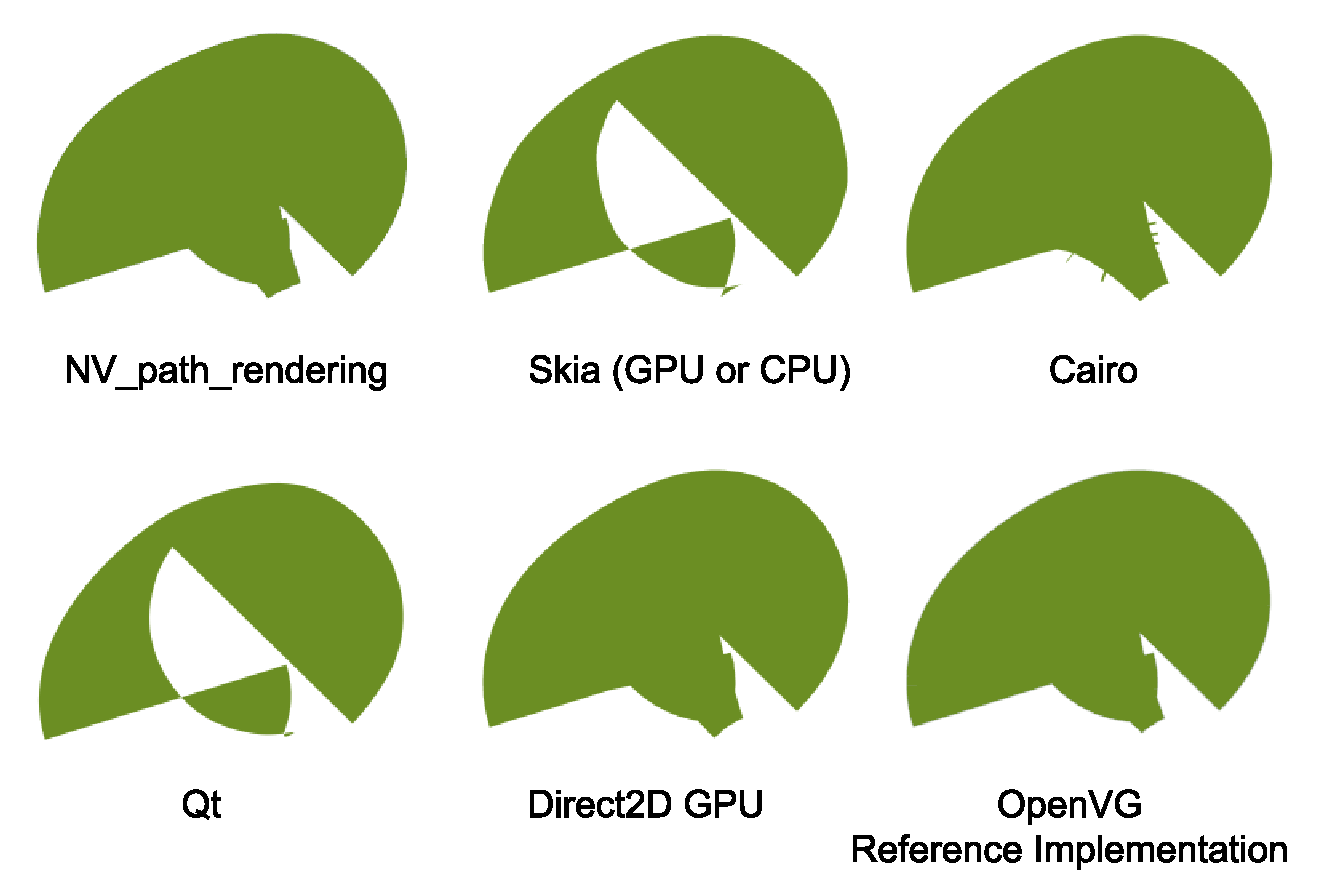
\includegraphics[width=\columnwidth]{stroke_quality.eps}}
  \center{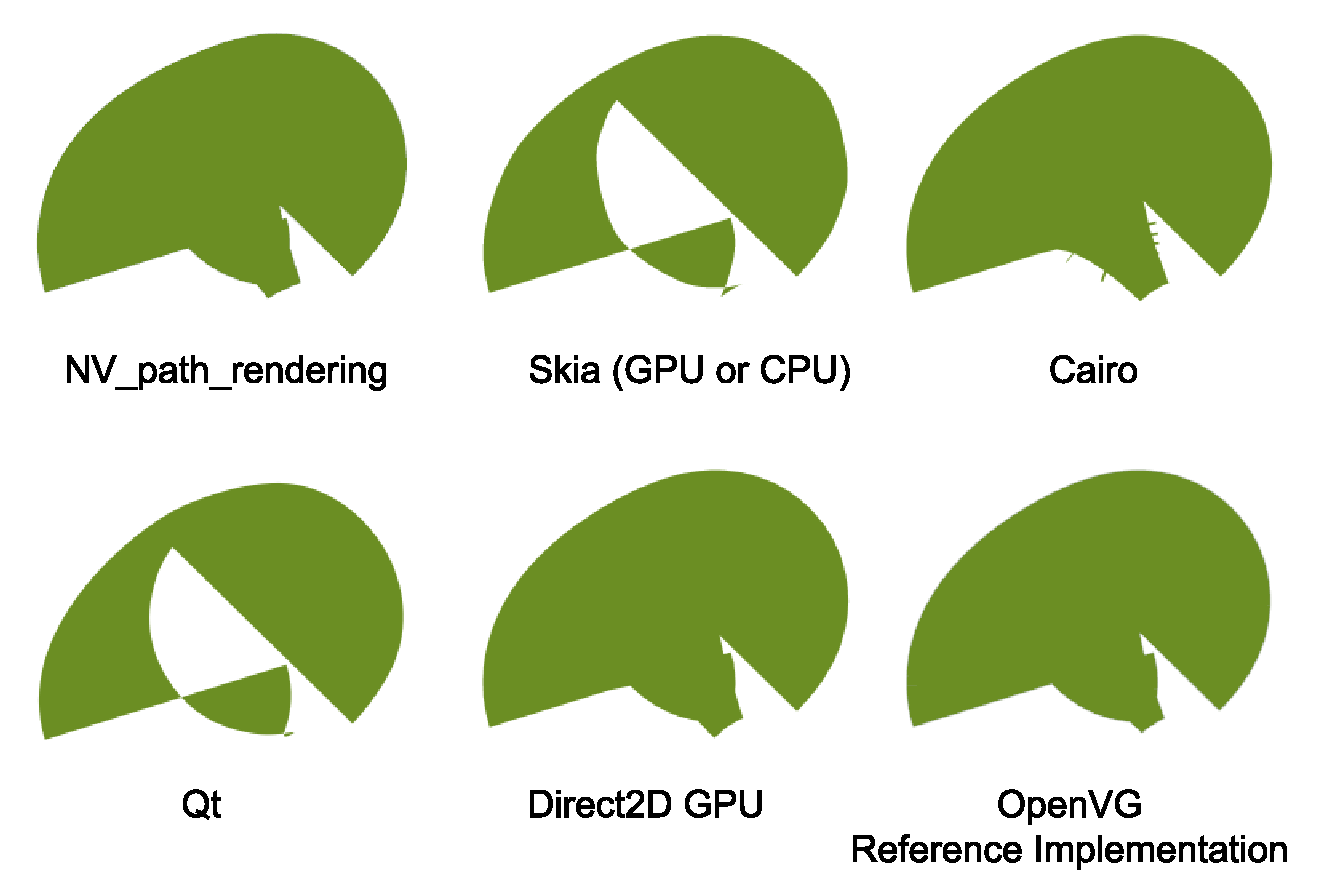
\includegraphics[width=3.1in]{stroke_quality.eps}}
  \caption{\label{fig:stroke-quality} Various path rendering
  implementations drawing a difficult cubic B\'{e}zier curve (the
  centurion head).}
\end{figure}

For stroking, our quadratic B\'{e}zier stroke discard shader is
mathematically consistent with the sweep of an orthogonal pen traversing
the path's trajectory.  In Figure \ref{fig:stroke-quality} we compare
our very fast stroking result to alternatives that are generally
substantially slower on a difficult cubic B\'{e}zier stroke test case.
Notice three path rendering implementation get this test case quite
wrong---whereas {\tt NV\_path\_rendering} matches the OpenVG reference
implementation and Direct2D version.
 
\subsubsection{Conflation Avoidance}

Conflation is an artifact in path rendering systems that occurs when
coverage (a Boolean concept) is {\em conflated} with opacity.  This generally
occurs when sub-pixel coverage is converted to a fractional value and
multiplied into the alpha color component for compositing.  While this
approach is standard practice, it can result in noticeably incorrect
colors.

Conflation is particularly noticeable when two opaque paths {\em exactly} seam
at a shared boundary.  Say path A covers 40\% of the pixel and an adjacent
path B covers the other 60\%.  But if A is drawn first, the pixel picks
up 40\% of A's color and 60\% of the background color.  Now when B is
drawn, the pixel gets 60\% of B's color and 40\% of the combination of
40\% of A's color and 60\% of the background color.  The result is some
fraction of the background color has leaked into the pixel when a more
accurate assessment of coverage would have no background color.

Flash content is particularly prone to conflation artifacts because path
edges are typically authored for exact sharing of edges.  Adobe's Flash
player specifically works to avoid conflation artifacts.  This is possible
because Flash player has complete knowledge of all the paths in a Flash
shape and how those path edges are shared.  Exact sharing of edges is
helpful from a content creation standpoint because a shared edge can be
stored once and used by two paths (more compact) and reduces the overall
layered depth complexity of the scene by avoiding overlaps.
Because {\tt NV\_path\_rendering} maintains distinct sub-pixel color
samples, the scene in Figure \ref{fig:conflation-artifacts} renders free
of conflation artifacts.

\begin{figure}[tb]
  %\center{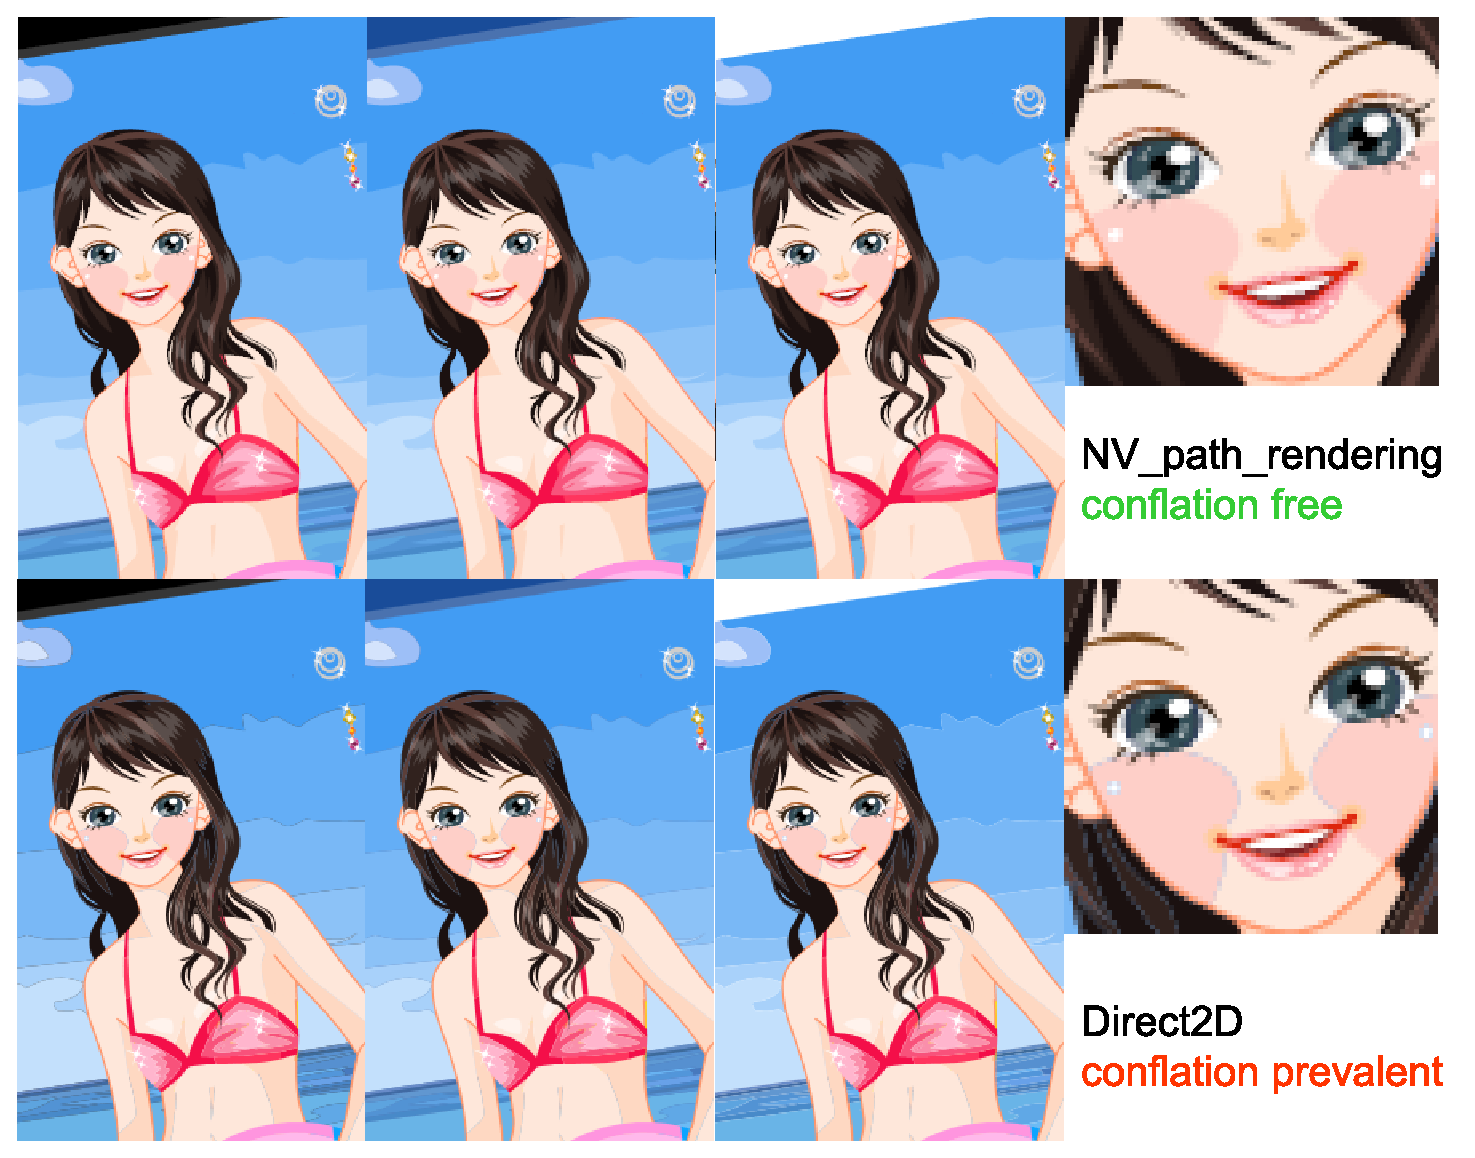
\includegraphics[width=\columnwidth]{conflation_artifacts.eps}}
  \center{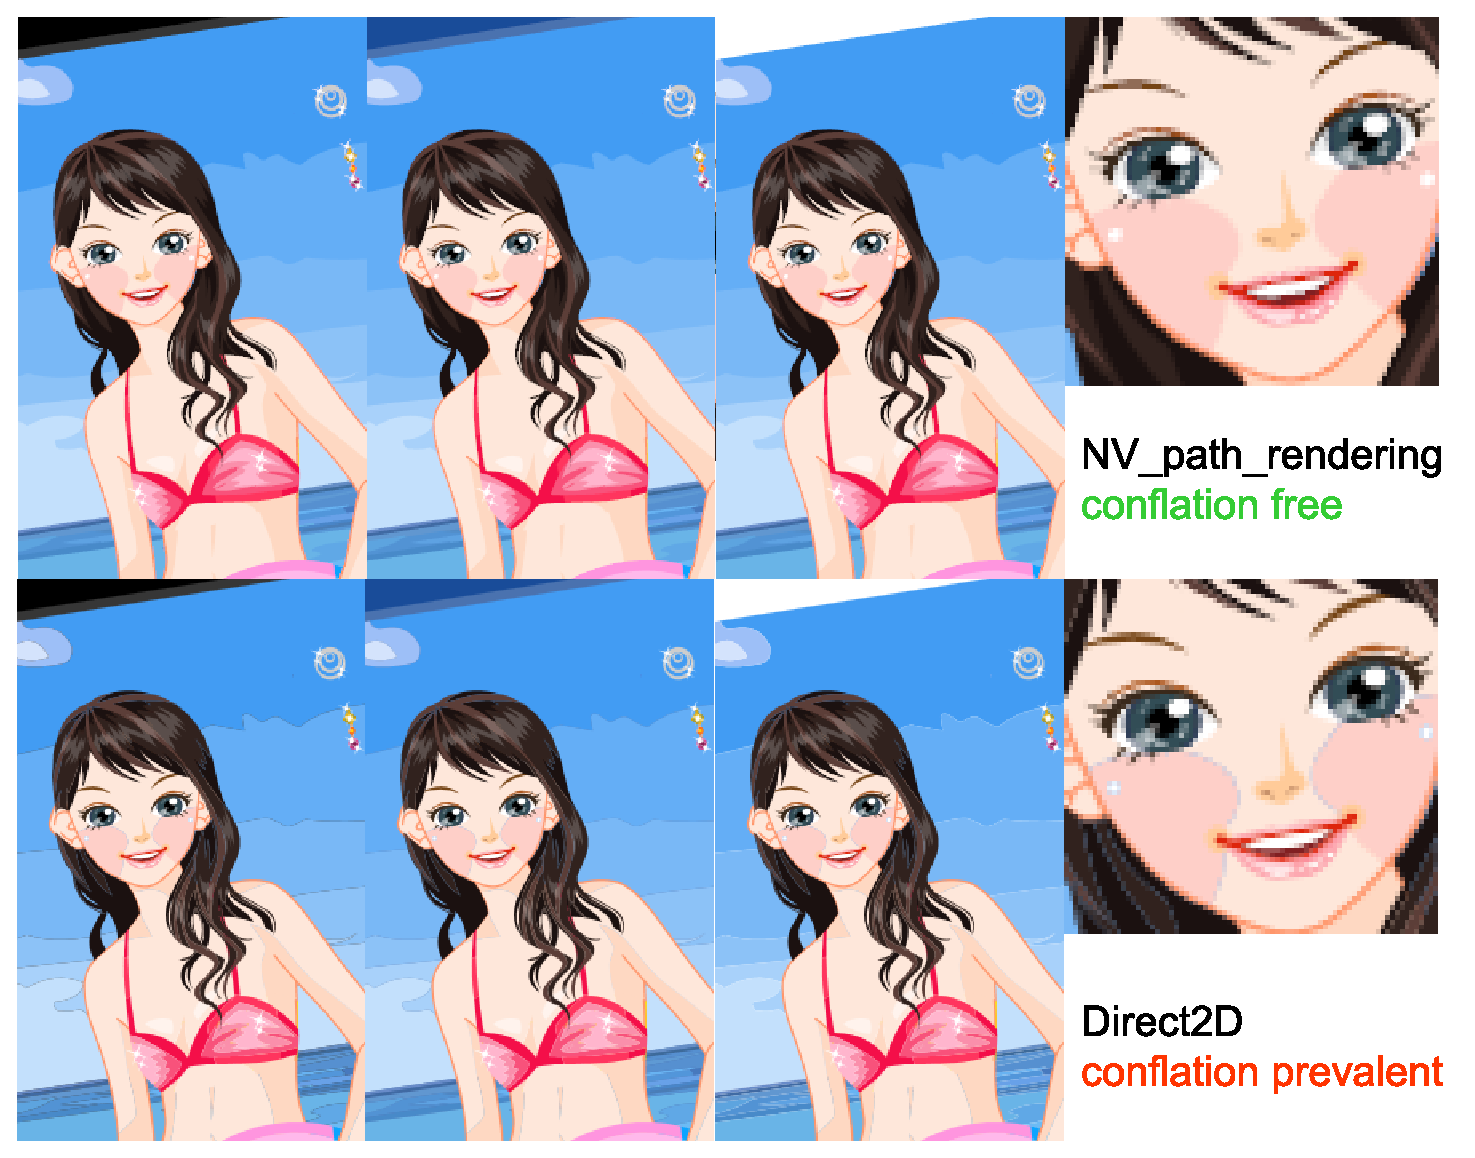
\includegraphics[width=3.3in]{conflation_artifacts.eps}}
  \caption{\label{fig:conflation-artifacts} Flash scene with shared edges.
  {\tt NV\_path\_rendering} shows no conflation while Direct2D (and Cairo,
  Skia, Qt, and OpenVG) shows conflation.  Upper left corner shows the
  background clear color; conflation is tinted by this color in the
  bottom scenes.  Notice the conflated blue tint on the girl's cheek.}
\end{figure}
 
\subsection{Performance}
\label{sec-performance}

The rendering performance of {\tt NV\_path\_rendering} scales with
GPU performance.  Because the baked paths reside on the GPU and are
resolution-independent, once baked, path rendering performance is
decoupled from CPU performance.
Figure \ref{fig:nvpr-performance}
charts the performance of {\tt NV\_path\_rendering} relative to
alternatives---including GPU-accelerated alternatives such as Direct2D and Skia's Ganesh approach.

Our performance advantage is attributable to the overall rendering
and shading performance of our underlying GPUs.  Several aspects are
particularly noteworthy.  Our underlying GPUs support a fast stencil
culling mode so hundreds of pixels can be culled in a single clock if a
coarse grain test can determine the stencil test for all the pixels would
fail.  This mitigates much of what might otherwise seem very inefficient
about the ``stencil, then cover'' approach.  Also stencil processing
generally is very well optimized.  The 8-bit memory transactions during
the stencil and cover steps can often run at memory bus saturating rates.
Our OpenGL driver implementation makes use of a configurable front-end
processor within the GPU---not otherwise accessible to applications---to
transition quickly between the stencil step and cover step and back.  This
avoids the driver performing expensive revalidations of CPU-managed
state so our rendering stays GPU-limited rather than CPU-bottlenecked,
even when presented with otherwise overwhelming numbers of small paths.

\subsection{New Functionality}
\label{sec:newfunc}

Because {\tt NV\_path\_rendering} is integrated into the OpenGL pipeline
and the coverage information is accessible through the stencil buffer,
we are able to implement unconventional algorithms such as mixing path
rendering with arbitrary 3D graphics.

\begin{figure}[bt]
  %\center{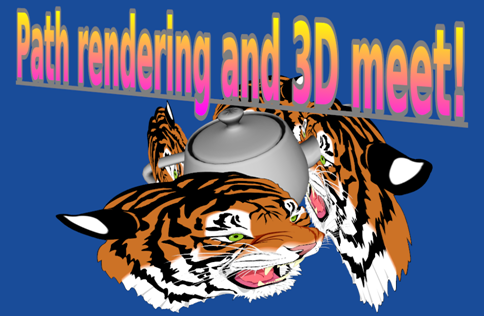
\includegraphics[width=\columnwidth]{tiger3d.png}}
  \center{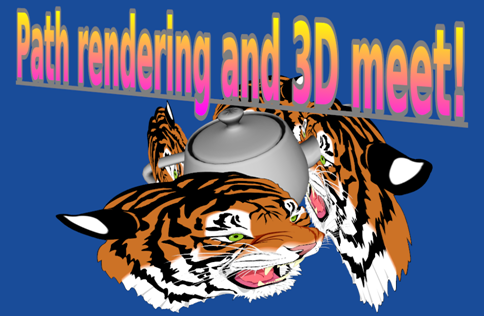
\includegraphics[width=3.3in]{tiger3d.png}}
  \caption{\label{fig:tiger3d} Mixing 3D and path rendering in a single
  window.}
\end{figure}

Figure \ref{fig:tiger3d} demonstrates an example of this capability.
No textures are used in this scene.  Arbitrary zooming into the tigers'
detail is supported.  Notice how the tigers properly occlude each other
and the teapot.  Due to the perspective 3D view, the path rendering is
properly rendered in perspective as well.




\section{Future Work}
\label{sec:future}

We believe our performance can be further improved.  We are investigating
hardware improvements to mitigate some of the memory bandwidth expense
involved in our underlying stencil-based algorithms.  In particular,
we are seeking to reduce the GPU memory footprint.

Web browser architecture should change to incorporate GPU-accelerated
path rendering.  Today web browsers
respecify paths every time a web page with path content is re-rendered
assuming respecifying paths is cheap relative to the expense of rendering them.
When path rendering is fully GPU-accelerated, a retained model of
rendering is more appropriate and  efficient.  We believe web browsers
should behave more like video games in this respect to exploit the GPU.

Mobile devices are power constrained so off-loading path rendering to
a graphics processor designed for efficient pixel processing
makes good sense.  Mobile devices in particular prize a low-latency
experience for the user so the sooner the device can complete its
resolution-independent 2D rendering, the better the user experience and
the sooner the device can power down to a low power state.




\section*{Acknowledgements}

Michael Toksvig corrected Mark's 3D bigotry and insisted 2D rendering deserved acceleration.
Chris Dalton assisted building our test bed.
Tero Karras provided crucial math insights.
Barthold Lichtenbelt supported this work throughout.


\pdfbookmark[1]{References}{bkmk:references}
\bibliographystyle{acmsiggraph}
%\nocite{*}  % include references not cited in the paper
\bibliography{gpupathrender}


\end{document}

% end
